% !TEX program = pdflatex
% Statistical Pharmacology via Kakutani Dichotomy III
% Companion computations: code/exp03_spectral_kakutani_criticality.py, code/paper03_compute_tables.py
\documentclass[11pt,reqno]{amsart}

\usepackage[T1]{fontenc}
\usepackage[utf8]{inputenc}
\usepackage{lmodern}
\usepackage[a4paper,margin=27mm]{geometry}
\usepackage{amsmath,amssymb,amsthm,mathtools}
\usepackage{booktabs}
\usepackage{graphicx}
\graphicspath{{./}{../figures/}}
\usepackage{array}
\usepackage{microtype}
\usepackage{enumitem}
\usepackage{xcolor}
\usepackage[colorlinks=true,linkcolor=blue!60!black,citecolor=blue!60!black,urlcolor=blue!60!black]{hyperref}

\theoremstyle{plain}
\newtheorem{theorem}{Theorem}[section]
\newtheorem{lemma}[theorem]{Lemma}
\newtheorem{proposition}[theorem]{Proposition}
\newtheorem{corollary}[theorem]{Corollary}
\theoremstyle{definition}
\newtheorem{definition}[theorem]{Definition}
\theoremstyle{remark}
\newtheorem{remark}[theorem]{Remark}
\numberwithin{equation}{section}

\DeclareMathOperator{\Tr}{Tr}
\DeclareMathOperator{\diag}{diag}
\DeclareMathOperator{\GL}{GL}
\DeclareMathOperator{\Or}{O}
\DeclareMathOperator{\SO}{SO}
\newcommand{\dd}{\mathrm{d}}
\newcommand{\Dcov}{D_{\mathrm{cov}}}
\newcommand{\Dcomm}{D_{\mathrm{comm}}}
\newcommand{\Drot}{D_{\mathrm{rot}}}
\newcommand{\Dtail}{D_{\mathrm{tail}}}
\newcommand{\gnaive}{\gamma_{\mathrm{naive}}}
\newcommand{\gtail}{\gamma_{\mathrm{tail}}}
\newcommand{\geff}{\gamma_{\mathrm{eff}}}
\newcommand{\Rr}{\mathbb{R}}
\newcommand{\Nn}{\mathbb{N}}
\newcommand{\PA}{P_{A}}
\newcommand{\PB}{P_{B}}
\newcommand{\CA}{C_A}
\newcommand{\CB}{C_B}
\newcommand{\PN}{\mathcal{P}_N}
\newcommand{\RMSD}{\mathrm{RMSD}}
\newcommand{\RMSF}{\mathrm{RMSF}}
\newcommand{\gEM}{\gamma_{\mathrm{EM}}}

\renewcommand{\abstractname}{Summary}

\title[Spectral Kakutani--Feldman--H\'ajek criticality]{Spectral Kakutani--Feldman--H\'ajek Criticality of Correlated Conformational Modes:\\ Mode Amplitude Perturbation, Iso-Spectral Givens Rotation, and Tail-Increment Finite-Size Elimination}

\author[Z. Chen]{Zhengyi Chen}
\address{Guangxi Key Laboratory of Drug Discovery and Optimization, School of Pharmacy, Guilin Medical University, Guilin 541199, P.~R. China}
\email{chenzhengyi@glmc.edu.cn}

\author[R. Chen]{Ruqing Chen}
\address{GUT Geoservice Inc., Montreal, Qu\'ebec, Canada}
\email{ruqing@hotmail.com}

\thanks{DOI: \href{https://doi.org/10.5281/zenodo.23015709}{10.5281/zenodo.23015709}. Sources, code and data: \url{https://github.com/Ruqing1963/kakutani-statistical-pharmacology-III} (see the Reproducibility paragraph of \S6). Papers I and II of the series are \cite{ChenChen2026I,ChenChen2026II}.}
\thanks{This project was supported by the National Natural Science Foundation of China (No.~22464010), the Guangxi Natural Science Foundation of China (No.~2025GXNSFAA069294), and the 2025 Bagui Youth Top Talent Project.}
\date{28 September 2026}

\subjclass[2020]{Primary 60G15, 92C40; Secondary 15B48, 53C35, 11M06, 62B10}
\keywords{Kakutani dichotomy, Feldman--H\'ajek theorem, Bhattacharyya distance, covariance spectrum, Givens rotation, symmetric positive definite cone, geodesic coordinates, Euler--Maclaurin summation, finite-size scaling, cryptic allostery}

\begin{document}

\begin{abstract}
Paper II of this series \cite{ChenChen2026II} decomposed the covariance part of the correlated Kakutani index of two Gaussian conformational ensembles into a commuting amplitude part and a non-commuting rotation part, $\Dcov=\Dcomm+\Drot$, and closed with the question of what happens when a ligand's effect on the collective modes decays along the mode index. This paper answers it. Two spectral perturbation mechanisms are defined on the cone $\PN$ of positive definite matrices: \emph{mode amplitude perturbation} (Mechanism~A), $\lambda^{(B)}_i=\lambda^{(A)}_i(1+c\,i^{-\alpha_\lambda})$ in a common eigenbasis, whose exact per-mode contribution is $\tfrac12\ln\frac{1+\delta/2}{\sqrt{1+\delta}}=\sum_{k\ge2}a_k\delta^k$ with $a_k=(-1)^k(1-2^{1-k})/(4k)$; and \emph{iso-spectral Givens rotation} (Mechanism~B), $\Lambda_A=\Lambda_B$ with the $k$-th adjacent pair of modes of anisotropy ratio $r$ rotated by $\theta_k=c_\theta k^{-\alpha_\theta}$, whose exact per-pair contribution is $\tfrac12\ln[1+\kappa(r)\sin^2\theta_k]$, $\kappa(r)=(r-1)^2/(4r)$. Both are normalised to the leading coefficient $A=0.0100$ of Paper~I. Theorem~\ref{thm:threeregime} gives the unified three-regime Euler--Maclaurin asymptotics of $\Dcov(N)$ for both mechanisms, with the limit constants in closed form, and the Feldman--H\'ajek dichotomy at $\alpha_c=\tfrac12$ for each mechanism separately; the predictions agree with the numerical experiment to $3\times10^{-12}$ or better at $N\ge100$ and to $10^{-8}$ at $N=10$. Theorem~\ref{thm:tail} proves that the doubling tail increment $\Dtail(N)=\Dcov(2N)-\Dcov(N)$ annihilates the Euler--Maclaurin constant $A\zeta(2\alpha)$, so that its regression exponent $\gtail(\alpha)$ equals $1-2\alpha$ on the whole range $0<\alpha<1$, including the negative subcritical values, and $\gtail^+=\max(\gtail,0)$ is the sharp phase curve; the bias of the naive exponent at $\alpha=0.45$ falls from $+0.073$ to $+0.003$ (A) and from $+0.062$ to $+0.0001$ (B). Theorem~\ref{thm:refined} gives the refined finite-size formula that reproduces the naive exponent to four decimals ($0.1729$ at $\alpha=0.45$, where Paper~I's two-term formula gives $0.1601$). Theorem~\ref{thm:parity} explains the residual difference between the two mechanisms by the geometry of $\PN$: in the geodesic coordinate $\eta_i=\ln(\lambda^{(B)}_i/\lambda^{(A)}_i)$ the per-mode divergence $\tfrac12\ln\cosh(\eta_i/2)$ is even, the odd terms of Mechanism~A are the curvature of the Euclidean coordinate $\delta_i=e^{\eta_i}-1$, and the resulting shift $\Delta\gtail=\alpha c\,\frac{1-2\alpha}{1-3\alpha}\frac{2^{1-3\alpha}-1}{2^{1-2\alpha}-1}N^{-\alpha}$ is verified; the geodesic variant $\lambda^{(B)}_i=\lambda^{(A)}_ie^{c\,i^{-\alpha_\lambda}}$ and the Givens mechanism, both even, give $\gtail(0.45)=+0.1001$. Theorem~\ref{thm:phase} establishes the joint $(\alpha_\lambda,\alpha_\theta)$ phase diagram: the infinite ensembles are equivalent iff $\min(\alpha_\lambda,\alpha_\theta)>\tfrac12$, with effective exponent $\max(1-2\min(\alpha_\lambda,\alpha_\theta),0)$, confirmed on a $19\times19$ grid with no misclassified point, and Corollary~\ref{cor:crossover} gives the finite-$N$ exponent on that grid as the Boltzmann-type convex combination of two power laws, reproducing all $361$ measured values to $4\times10^{-4}$; the rotation-only singular phase is the iso-spectral signature of cryptic allostery. The paper closes with an assessment and with the empirical-covariance (Marchenko--Pastur) problem for the next step.
\end{abstract}

\maketitle
\tableofcontents

%%%%%%%%%%%%%%%%%%%%%%%%%%%%%%%%%%%%%%%%%%%%%%%%%%%%%%%%%%%%%%%%%%%%%%%%%%%%%%%
\section{Introduction and summary of main results}
\label{sec:intro}

\subsection*{What Papers I and II established}
Paper~I \cite{ChenChen2026I} modelled a protein with $N$ independent two-state switches and two ligands as product Bernoulli measures, defined the marginal drug Kakutani index $K_N=\sum_{i\le N}h_i$ (a sum of local squared Hellinger distances), and proved for the power-law shift $q_i=p+c\,i^{-\alpha}$ the trichotomy: $K_N\sim AN^{1-2\alpha}/(1-2\alpha)$ for $\alpha<\tfrac12$, $K_N=A(\ln N+\gEM)+O(1)$ at $\alpha=\tfrac12$, $K_N\to K_\infty<\infty$ for $\alpha>\tfrac12$, with $A=c^2/(4p(1-p))=0.0100$; by Kakutani's theorem \cite{Kakutani1948} the infinite ensembles are singular in the first two cases and equivalent in the third. It also isolated a finite-size artefact: the exponent read from a regression of $\ln K_N$ on $\ln N$ over $[10^3,10^5]$ is $\geff=(1-2\alpha)/\bigl(1+(1-2\alpha)\zeta(2\alpha)N^{2\alpha-1}\bigr)$, and because $\zeta(2\alpha)\to-\infty$ as $2\alpha\to1$ the measured exponent at $\alpha=0.45$ is $0.161$ instead of $0.100$; the doubling estimator $K_{2N}-K_N$ removed the bias. Paper~II \cite{ChenChen2026II} replaced the product measures by Gaussian ensembles $\mathcal N(\mu_A,\CA)$, $\mathcal N(\mu_B,\CB)$, defined the correlated index as the Bhattacharyya distance $D_B=D_{\mathrm{mean}}+\Dcov$, proved the commuting--rotation decomposition
\begin{equation}\label{eq:decomp}
\Dcov=\Dcomm+\Drot,\qquad \Dcomm=\frac12\sum_{i=1}^N\ln\cosh\frac{\eta_i}{2},\quad \eta_i=\ln\frac{\lambda^{(B)}_i}{\lambda^{(A)}_i},\qquad \Drot\ge0,
\end{equation}
with $\Drot=0$ iff the covariances share an ordered eigenbasis, and showed for Kac--Murdock--Szeg\H{o} networks that the covariance term dominates the mean term ($99.95\%$) and diverges linearly in $N$ because the network change touches every mode with undiminished strength.

\subsection*{The three questions of this paper}
In a real protein an allosteric ligand reshapes strongly only the low-frequency collective modes; its effect on the high-frequency, localised modes decays with the mode index. This raises three questions.
\begin{enumerate}[label=(\arabic*),leftmargin=*]
\item Do the two parts of \eqref{eq:decomp}---a perturbation of the mode amplitudes (Mechanism~A) and an iso-spectral rotation of the mode directions (Mechanism~B, $\Lambda_A=\Lambda_B$)---each induce a Kakutani--Feldman--H\'ajek transition, and is the critical exponent again $\alpha_c=\tfrac12$?
\item Can a difference operator remove the Euler--Maclaurin constant $\zeta(2\alpha)$ at its root, so that at finite $N\le10^5$ the phase curve is the sharp kink $\max(1-2\alpha,0)$ and, at the same time, the negative tail exponent $1-2\alpha<0$ of the subcritical regime is measured?
\item Why, at $\alpha=0.45$, is the doubling-tail exponent of Mechanism~B equal to $+0.1001$ (error $10^{-4}$) while that of Mechanism~A is $+0.1028$ (shift $+0.0028$)?
\end{enumerate}
The answers are: yes, with $\alpha_c=\tfrac12$ for each mechanism separately (Theorem~\ref{thm:threeregime}); yes, the doubling tail increment (Theorem~\ref{thm:tail}), whose remaining finite-size residual is fully predicted by Theorem~\ref{thm:refined}; and because Mechanism~A is written in the Euclidean coordinate $\delta_i=\lambda^{(B)}_i/\lambda^{(A)}_i-1$ of the Riemannian symmetric space $\PN=\GL_N(\Rr)/\Or(N)$, whereas the Bhattacharyya divergence is an even function of the geodesic coordinate $\eta_i=\ln(1+\delta_i)$; the odd terms are the curvature of the pull-back, and they vanish for the geodesic variant of Mechanism~A and for the Givens rotation, whose angle is already a geodesic coordinate in $\SO(2)$ (Theorem~\ref{thm:parity}). Theorem~\ref{thm:phase} combines the two mechanisms into a joint phase diagram whose rotation-only singular quadrant is the mathematical form of cryptic, iso-spectral allostery.

\subsection*{Standing notation}
$\PN$ is the cone of symmetric positive definite $N\times N$ matrices. For $\CA,\CB\in\PN$, $S=\tfrac12(\CA+\CB)$ and
\[
\Dcov=\tfrac12\ln\det S-\tfrac14\ln\det\CA-\tfrac14\ln\det\CB .
\]
$H_N(s)=\sum_{i\le N}i^{-s}$; $\zeta$ is the Riemann zeta function (meromorphic, simple pole at $1$); $\gEM=0.5772156649\ldots$. The regression window is $[10^3,10^5]$ with a sixty-point log-uniform grid and logarithmic centre $N_*=10^4$. The benchmark parameters are $c=0.40$ for Mechanism~A (so that $c^2/16=0.0100$), $r=3$ and $c_\theta=\sqrt{0.06}=0.2449490$ for Mechanism~B (so that $\kappa(3)c_\theta^2/2=0.0100$), and $A=0.0100$ denotes the common leading coefficient.

%%%%%%%%%%%%%%%%%%%%%%%%%%%%%%%%%%%%%%%%%%%%%%%%%%%%%%%%%%%%%%%%%%%%%%%%%%%%%%%
\section{Spectral and rotational perturbation mechanisms on the SPD cone}
\label{sec:mechanisms}

\begin{definition}[Mechanism A: collective mode amplitude scaling]\label{def:A}
Let $\CA=Q\Lambda_AQ^{\mathsf T}$ with $\Lambda_A=\diag(\lambda^{(A)}_1\ge\dots\ge\lambda^{(A)}_N>0)$, and let $\CB=Q\Lambda_BQ^{\mathsf T}$ have the same eigenvectors with
\begin{equation}\label{eq:mechA}
\lambda^{(B)}_i=\lambda^{(A)}_i(1+\delta_i),\qquad \delta_i=c\,i^{-\alpha_\lambda},\quad 0<c<1,\ \alpha_\lambda>0 .
\end{equation}
Then $\Drot=0$ and $\Dcov(N)=\Dcomm(N)=\sum_{i\le N}d_{\mathrm{cov},i}$ with $d_{\mathrm{cov},i}=\tfrac12\ln\frac{\lambda^{(A)}_i+\lambda^{(B)}_i}{2\sqrt{\lambda^{(A)}_i\lambda^{(B)}_i}}$. The \emph{geodesic variant} (Mechanism~A-geo) replaces \eqref{eq:mechA} by $\lambda^{(B)}_i=\lambda^{(A)}_ie^{c\,i^{-\alpha_\lambda}}$, i.e.\ $\eta_i=c\,i^{-\alpha_\lambda}$.
\end{definition}

\begin{proposition}[Exact per-mode contribution of Mechanism A]\label{prop:A}
For $\delta\in(-1,1)$,
\begin{equation}\label{eq:dA}
d_{\mathrm{cov}}(\delta)=\frac12\ln\frac{1+\delta/2}{\sqrt{1+\delta}}=\sum_{k\ge2}a_k\delta^k,\qquad a_k=\frac{(-1)^k\bigl(1-2^{1-k}\bigr)}{4k},
\end{equation}
so that
\begin{equation}\label{eq:dAexp}
d_{\mathrm{cov}}(\delta)=\frac{\delta^2}{16}-\frac{\delta^3}{16}+\frac{7\delta^4}{128}-\frac{3\delta^5}{64}+\frac{31\delta^6}{768}-\frac{9\delta^7}{256}+O(\delta^8).
\end{equation}
The series converges absolutely for $|\delta|<1$, and $|a_k|\le1/(4k)$.
\end{proposition}

\begin{proof}
With $\lambda^{(B)}=\lambda^{(A)}(1+\delta)$, $\frac{\lambda^{(A)}+\lambda^{(B)}}{2\sqrt{\lambda^{(A)}\lambda^{(B)}}}=\frac{2+\delta}{2\sqrt{1+\delta}}=\frac{1+\delta/2}{\sqrt{1+\delta}}$, which gives the closed form. Expanding, $\ln(1+\delta/2)=\sum_{k\ge1}(-1)^{k+1}\delta^k/(k2^k)$ and $\tfrac12\ln(1+\delta)=\sum_{k\ge1}(-1)^{k+1}\delta^k/(2k)$ for $|\delta|<1$, so
\[
d_{\mathrm{cov}}(\delta)=\frac12\sum_{k\ge1}\frac{(-1)^{k+1}}{k}\Bigl(\frac1{2^k}-\frac12\Bigr)\delta^k=\sum_{k\ge1}\frac{(-1)^k(2^{-1}-2^{-k})}{2k}\delta^k=\sum_{k\ge1}\frac{(-1)^k(1-2^{1-k})}{4k}\delta^k .
\]
The $k=1$ coefficient is $0$, and $a_2=\frac{1-1/2}{8}=\frac1{16}$, $a_3=-\frac{1-1/4}{12}=-\frac1{16}$, $a_4=\frac{1-1/8}{16}=\frac7{128}$, $a_5=-\frac{1-1/16}{20}=-\frac3{64}$, $a_6=\frac{1-1/32}{24}=\frac{31}{768}$, $a_7=-\frac{1-1/64}{28}=-\frac9{256}$. Absolute convergence for $|\delta|<1$ and the bound follow from $0<1-2^{1-k}<1$.
\end{proof}

\subsection*{On the coefficients}
The series \eqref{eq:dA} is alternating with closed-form coefficients $a_2=\tfrac1{16}$, $a_3=-\tfrac1{16}$, $a_4=\tfrac7{128}$, $a_5=-\tfrac3{64}$, $a_6=\tfrac{31}{768}$, $a_7=-\tfrac9{256}$; the companion script confirms them independently, the residual $\bigl(d_{\mathrm{cov}}-\sum_{k\le4}a_k\delta^k\bigr)/\delta^5$ tending to $-0.046875=-\tfrac3{64}$ as $\delta\to0$. The ratio $|a_{k+1}/a_k|=\frac{k}{k+1}\frac{1-2^{-k}}{1-2^{1-k}}\to1$, so the radius of convergence is exactly $1$: it is set by the algebraic branch point of $\sqrt{1+\delta}$ at $\delta=-1$, not by $\ln(1+\delta/2)$, whose singularity lies at $\delta=-2$. With $c=0.4$ the leading term is $c^2/16=0.0100=A$, the same prefactor as Paper~I, but the cubic term $-c^3/16=-0.0040$ is $40\%$ of it at $i=1$ and the series converges only geometrically with ratio $0.4$: Mechanism~A is a genuinely non-perturbative test of the $\alpha_c=\tfrac12$ law, and the odd terms will be seen to matter in Section~\ref{sec:tail}.

\begin{definition}[Mechanism B: iso-spectral Givens mode rotation]\label{def:B}
Let $\Lambda_A=\Lambda_B=\Lambda$ (every amplitude unchanged), and group the modes into adjacent pairs $(2k-1,2k)$, $k=1,\dots,N$ (dimension $2N$), with anisotropy ratio $r=\lambda_{2k-1}/\lambda_{2k}>1$. Let $\CA=\Lambda$ (block diagonal with blocks $\diag(\lambda_{2k-1},\lambda_{2k})$) and let $\CB$ be obtained by rotating the $k$-th block by $R(\theta_k)\in\SO(2)$,
\begin{equation}\label{eq:mechB}
\CB^{(k)}=R(\theta_k)\diag(\lambda_{2k-1},\lambda_{2k})R(\theta_k)^{\mathsf T},\qquad \theta_k=c_\theta k^{-\alpha_\theta}.
\end{equation}
Then $\Dcomm=0$ identically and $\Dcov(N)=\Drot(N)=\sum_{k\le N}d_{\mathrm{rot},k}$. Here $N$ counts rotated pairs.
\end{definition}

\begin{proposition}[Exact per-pair contribution of Mechanism B]\label{prop:B}
For every $\theta$,
\begin{equation}\label{eq:dB}
d_{\mathrm{rot}}(\theta)=\frac12\ln\bigl[1+\kappa(r)\sin^2\theta\bigr],\qquad \kappa(r)=\frac{(r-1)^2}{4r},
\end{equation}
an even function of $\theta$, with
\begin{equation}\label{eq:dBexp}
d_{\mathrm{rot}}(\theta)=\frac{\kappa}{2}\theta^2-\frac{\kappa(2+3\kappa)}{12}\theta^4+O(\theta^6).
\end{equation}
For $r=3$, $\kappa=\tfrac13$ and $d_{\mathrm{rot}}(\theta)=\theta^2/6-\theta^4/12+O(\theta^6)$.
\end{proposition}

\begin{proof}
Write the block as $\CA=\diag(a,b)$, $a=\lambda_{2k-1}$, $b=\lambda_{2k}$, and $\CB=R\CA R^{\mathsf T}$ with $R=\begin{psmallmatrix}\cos\theta&-\sin\theta\\ \sin\theta&\cos\theta\end{psmallmatrix}$; abbreviate $C=\cos\theta$, $S=\sin\theta$. Then $\CB=\begin{psmallmatrix}aC^2+bS^2&(a-b)CS\\ (a-b)CS&aS^2+bC^2\end{psmallmatrix}$ and the block of $\frac12(\CA+\CB)$ has determinant
\begin{align*}
\tfrac14\bigl[(a+aC^2+bS^2)(b+aS^2+bC^2)-(a-b)^2C^2S^2\bigr]&=\tfrac14\bigl[(a^2+b^2)S^2+2ab(1+C^2)\bigr]\\
&=ab\Bigl[1+\frac{(a-b)^2}{4ab}S^2\Bigr],
\end{align*}
where the middle equality expands the product, uses $C^2+S^2=1$ and cancels the $(a-b)^2C^2S^2$ terms, and the last uses $1+C^2=2-S^2$. Since $\det\CA=\det\CB=ab$, $d_{\mathrm{rot}}=\frac12\ln\det\frac{\CA+\CB}{2}-\frac14\ln(ab)^2=\frac12\ln\bigl[1+\frac{(a-b)^2}{4ab}S^2\bigr]$, which is \eqref{eq:dB} with $\kappa=(a-b)^2/(4ab)=(r-1)^2/(4r)$. Evenness is that of $\sin^2$. For the expansion, $\sin^2\theta=\theta^2-\theta^4/3+O(\theta^6)$ and $\frac12\ln(1+u)=\frac u2-\frac{u^2}4+O(u^3)$ with $u=\kappa\sin^2\theta$ give $\frac\kappa2\theta^2-\frac\kappa6\theta^4-\frac{\kappa^2}4\theta^4+O(\theta^6)$, and $\frac\kappa6+\frac{\kappa^2}4=\frac{\kappa(2+3\kappa)}{12}$.
\end{proof}

\begin{remark}[Normalisation and the geometry of $\PN$]
With $r=3$ and $c_\theta^2=0.06$ the leading coefficient is $\kappa c_\theta^2/2=0.0100=A$, and the fourth-order coefficient is $-\kappa(2+3\kappa)c_\theta^4/12=-3.0\times10^{-4}$, three orders of magnitude below the leading one: Mechanism~B is perturbative where Mechanism~A is not. The two mechanisms are the two factors of the polar decomposition of a change of covariance on $\PN=\GL_N(\Rr)/\Or(N)$ \cite{Bhatia2007,Pennec2006}: in the common eigenbasis the affine-invariant geodesic from $\CA$ to $\CB$ is $\Lambda_A^{1/2}\exp(t\,\diag(\eta_i))\Lambda_A^{1/2}$, with $\eta_i=\ln(\lambda^{(B)}_i/\lambda^{(A)}_i)$ the geodesic coordinates, while a rotation of the eigenbasis moves along the orbit of $\Or(N)$, whose geodesic coordinate is the angle $\theta\in\mathfrak{so}(2)$. Mechanism~A-geo and Mechanism~B are perturbations in geodesic coordinates; Mechanism~A is a perturbation in the Euclidean coordinate $\delta=e^\eta-1$. Section~\ref{sec:tail} shows that this distinction is exactly what the finite-size exponents see.
\end{remark}

%%%%%%%%%%%%%%%%%%%%%%%%%%%%%%%%%%%%%%%%%%%%%%%%%%%%%%%%%%%%%%%%%%%%%%%%%%%%%%%
\section{Spectral Feldman--H\'ajek dichotomy and three-regime Euler--Maclaurin asymptotics}
\label{sec:asymptotics}

We use the Euler--Maclaurin expansion of the generalised harmonic numbers in the form proved in Paper~I: for $s>0$, $s\ne1$,
\begin{equation}\label{eq:EM}
\begin{gathered}
H_N(s)=\frac{N^{1-s}}{1-s}+\zeta(s)+\frac{N^{-s}}2-\frac{sN^{-s-1}}{12}+O(N^{-s-3}),\\
H_N(1)=\ln N+\gEM+\frac1{2N}-\frac1{12N^2}+O(N^{-4}),
\end{gathered}
\end{equation}
where for $0<s<1$ the constant is the analytic continuation of $\zeta$ (negative on $(0,1)$, with $\zeta(s)=\frac1{s-1}+\gEM+O(s-1)$).

\begin{theorem}[Unified three-regime asymptotics for mode amplitude and mode rotation]\label{thm:threeregime}
Let $\alpha>0$ and write the per-index contribution of either mechanism as a convergent power series in the perturbation amplitude, $d(u)=\sum_{k\in\mathcal K}a_ku^k$ with $u_i=c\,i^{-\alpha}$: for Mechanism~A, $\mathcal K=\{2,3,4,\dots\}$ and $a_k$ as in \eqref{eq:dA}; for Mechanism~A-geo, $\mathcal K=\{2,4,6,\dots\}$ with $g_2=\tfrac1{16}$, $g_4=-\tfrac1{384}$, $g_6=\tfrac1{5760}$, \dots; for Mechanism~B, $\mathcal K=\{2,4,6,\dots\}$ with $b_2=\kappa/2$, $b_4=-\kappa(2+3\kappa)/12$, \dots\ and $c=c_\theta$. Then for every $N$,
\begin{equation}\label{eq:Dseries}
\Dcov(N)=\sum_{k\in\mathcal K}a_kc^k\,H_N(k\alpha),
\end{equation}
and, with $A:=a_2c^2$ and $\alpha\notin\{1/k:k\in\mathcal K\}$ unless stated:
\begin{enumerate}[label=\textup{(\arabic*)}]
\item \textbf{Supercritical regime, $0<\alpha<\tfrac12$.}
\begin{equation}\label{eq:super}
\Dcov(N)=\sum_{k\in\mathcal K,\ k\alpha<1}a_kc^k\frac{N^{1-k\alpha}}{1-k\alpha}+C(\alpha)+O\bigl(N^{-2\alpha}\bigr)+O\bigl(N^{1-k_0\alpha}\bigr),\qquad C(\alpha)=\sum_{k\in\mathcal K}a_kc^k\zeta(k\alpha),
\end{equation}
where $k_0=\min\{k\in\mathcal K:k\alpha>1\}$; the leading term is $\frac{A}{1-2\alpha}N^{1-2\alpha}\to\infty$. (If $k\alpha=1$ for some $k$, the corresponding term is $a_kc^k(\ln N+\gEM)$.)
\item \textbf{Critical regime, $\alpha=\tfrac12$.}
\begin{equation}\label{eq:crit}
\Dcov(N)=A\ln N+C_{\mathrm{crit}}+O\bigl(N^{-\beta}\bigr),\qquad C_{\mathrm{crit}}=A\gEM+\sum_{k\in\mathcal K,\ k\ge3}a_kc^k\zeta(k/2),
\end{equation}
with $\beta=\tfrac12$ for Mechanism~A (from the $k=3$ term) and $\beta=1$ for the even mechanisms.
\item \textbf{Subcritical regime, $\alpha>\tfrac12$.}
\begin{equation}\label{eq:sub}
\begin{gathered}
D_\infty(\alpha)=\lim_{N\to\infty}\Dcov(N)=\sum_{k\in\mathcal K}a_kc^k\zeta(k\alpha)<\infty,\\
\Dcov(N)=D_\infty(\alpha)-\frac{A}{2\alpha-1}N^{1-2\alpha}+O\bigl(N^{1-k_1\alpha}\bigr),
\end{gathered}
\end{equation}
$k_1$ the second element of $\mathcal K$.
\end{enumerate}
Consequently, for each mechanism separately, the infinite-dimensional Gaussian ensembles satisfy $\PA\perp\PB$ for $\alpha\le\tfrac12$ and $\PA\sim\PB$ for $\alpha>\tfrac12$: $\alpha_c=\tfrac12$ is the critical exponent of the mode amplitudes and of the mode orientations alike.
\end{theorem}

\begin{proof}
For Mechanism~A, $u_i=\delta_i=c\,i^{-\alpha}\le c<1$, so \eqref{eq:dA} converges absolutely at every $i$ and $\Dcov(N)=\sum_{i\le N}\sum_ka_k\delta_i^k=\sum_ka_kc^k\sum_{i\le N}i^{-k\alpha}$, the interchange being justified by absolute convergence ($\sum_k|a_k|c^k<\infty$); this is \eqref{eq:Dseries}. For Mechanism~B, $d_{\mathrm{rot}}(\theta)=\frac12\ln(1+\kappa\sin^2\theta)$ is even and analytic in $\theta$ with radius of convergence at least the distance to the nearest zero of $1+\kappa\sin^2\theta$, which is $|\theta|=\operatorname{arcsinh}(\kappa^{-1/2})>1$ for $\kappa=\tfrac13$; since $\theta_k\le c_\theta<1$ the same argument applies. For Mechanism~A-geo, $\frac12\ln\cosh(\eta/2)$ is even and entire in $\eta$ except at $\eta=\pm\mathrm i\pi$, and $\eta_i\le c<\pi$.

Insert \eqref{eq:EM} into \eqref{eq:Dseries}. (1) For $k\alpha<1$ the term $N^{1-k\alpha}/(1-k\alpha)$ grows; for $k\alpha>1$ it decays as $N^{1-k\alpha}$ (dominated by $k=k_0$); the constants assemble into $C(\alpha)$, which converges absolutely because $|\zeta(k\alpha)|$ is bounded for $k\alpha$ away from $1$ and $\sum|a_k|c^k<\infty$; the $N^{-k\alpha}/2$ terms are $O(N^{-2\alpha})$. Since all terms with $k\alpha<1$ have $1-k\alpha<1-2\alpha$ for $k\ge3$, the $k=2$ term leads. (2) At $\alpha=\tfrac12$ the $k=2$ term is $A(\ln N+\gEM)+O(N^{-1})$ and every $k\ge3$ term converges, with tail $O(N^{1-k/2})$; the largest tail is $k=3$ ($N^{-1/2}$) for Mechanism~A and $k=4$ ($N^{-1}$) for the even mechanisms. (3) For $\alpha>\tfrac12$ every $k\alpha>1$, each $H_N(k\alpha)\uparrow\zeta(k\alpha)$, and dominated convergence gives the limit; the finite-$N$ correction is dominated by the $k=2$ tail $-\frac{A}{2\alpha-1}N^{1-2\alpha}$, the next being $O(N^{1-k_1\alpha})$.

Singularity or equivalence: $\Dcov(N)$ is the Bhattacharyya distance of the $N$-dimensional (respectively $2N$-dimensional) projections, so the affinity of the projections is $e^{-\Dcov(N)}$; as in Paper~II the affinity of the infinite Gaussian measures is the limit of the projected affinities (martingale convergence of the density ratios, Kakutani's argument \cite{Kakutani1948}), hence zero iff $\Dcov(N)\to\infty$, and by Feldman--H\'ajek \cite{Feldman1958,Hajek1958} there is no third case. Here $\Dcov(N)\to\infty$ iff $\alpha\le\tfrac12$ by (1)--(3). Equivalently, $\Dcomm\asymp\sum\eta_i^2$ and $\Drot\asymp\sum\theta_k^2$ (Propositions~\ref{prop:A} and \ref{prop:B}), so the criterion is the square-summability $\sum_i\eta_i^2<\infty$ resp.\ $\sum_k\theta_k^2<\infty$, the spectral form of the Kakutani condition.
\end{proof}

\begin{remark}[Numerical values of the constants]\label{rem:constants}
The companion script evaluates \eqref{eq:Dseries}--\eqref{eq:sub} with forty series terms. At $\alpha=\tfrac12$: $C_{\mathrm{crit}}=-0.0028681714$ (A), $+0.0056633399$ (A-geo), $+0.0052868221$ (B); the measured regressions of $\Dcov$ on $\ln N$ give slopes $0.009954$, $0.009999$, $0.009999$ and intercepts $-0.002341$, $0.005672$, $0.005296$---the even mechanisms agree with $A=0.0100$ and $C_{\mathrm{crit}}$ to $10^{-5}$, while Mechanism~A's $N^{-1/2}$ correction from the $k=3$ term ($+\frac{c^3}{16}\cdot2N^{-1/2}=0.008N^{-1/2}$ inside the window) shifts its regression slope by $-5\times10^{-5}$ and its intercept by $+5\times10^{-4}$. The limits are $D_\infty(0.75)=0.0215672275$, $D_\infty(1)=0.0127838165$ (A); $0.0260443577$, $0.0163779007$ (A-geo); $0.0257702719$, $0.0161315225$ (B). The doubling increments at $\alpha=\tfrac12$ converge to $A\ln2=0.0069315$: measured $0.0069240$ (A, $N=10^5$, the deficit being the $k=3$ term) and $0.0069315$ (B). Tables~\ref{tab:benchA} and \ref{tab:benchB} compare the multi-term prediction with the measured $\Dcov(N)$: the agreement is $3\times10^{-12}$ or better for $N\ge100$ and $10^{-8}$ at $N=10$, where the truncation of the asymptotic expansion \eqref{eq:EM} after the $N^{-s-1}$ term is the limiting factor.
\end{remark}

%%%%%%%%%%%%%%%%%%%%%%%%%%%%%%%%%%%%%%%%%%%%%%%%%%%%%%%%%%%%%%%%%%%%%%%%%%%%%%%
\section{The doubling tail-increment operator and the geodesic parity theorem}
\label{sec:tail}

\begin{theorem}[Constant-term annihilation via the doubling tail increment]\label{thm:tail}
Let $\Dcov(N)=\sum_{k\in\mathcal K}a_kc^kH_N(k\alpha)$ be as in Theorem~\ref{thm:threeregime} and define the doubling tail increment
\begin{equation}\label{eq:Dtail}
\Dtail(N):=\Dcov(2N)-\Dcov(N)=\sum_{i=N+1}^{2N}d_i .
\end{equation}
Then, for every $\alpha\in(0,1)$ with $k\alpha\ne1$ for all $k\in\mathcal K$,
\begin{equation}\label{eq:Dtailasym}
\Dtail(N)=\sum_{k\in\mathcal K}a_kc^k\frac{(2N)^{1-k\alpha}-N^{1-k\alpha}}{1-k\alpha}+O(N^{-2\alpha})
=A\,\frac{2^{1-2\alpha}-1}{1-2\alpha}\,N^{1-2\alpha}\bigl[1+R_{\mathrm{sub}}(N)\bigr],
\end{equation}
where every constant $a_kc^k\zeta(k\alpha)$ has cancelled identically and
\begin{equation}\label{eq:Rsub}
R_{\mathrm{sub}}(N)=\frac{a_{k_1}c^{k_1}}{a_2c^2}\,\frac{1-2\alpha}{1-k_1\alpha}\,\frac{2^{1-k_1\alpha}-1}{2^{1-2\alpha}-1}\,N^{-(k_1-2)\alpha}+O\bigl(N^{-(k_2-2)\alpha}\bigr)+O(N^{-1}),
\end{equation}
$k_1<k_2$ the second and third elements of $\mathcal K$. Consequently the local exponent $\gtail(\alpha;N)=\dd\ln\Dtail/\dd\ln N$ satisfies
\begin{equation}\label{eq:gtaillimit}
\lim_{N\to\infty}\gtail(\alpha;N)=1-2\alpha\qquad\text{for all }\alpha\in(0,1)\setminus\{\tfrac12\},
\end{equation}
including the negative values $1-2\alpha<0$ of the subcritical regime, while at $\alpha=\tfrac12$, $\Dtail(N)\to A\ln2$ and $\gtail\to0$. Hence $\gtail^+(\alpha)=\max(\gtail(\alpha),0)\to\max(1-2\alpha,0)$: the doubling estimator recovers the sharp phase curve without the pole-induced rounding of the naive exponent.
\end{theorem}

\begin{proof}
Apply \eqref{eq:EM} at $2N$ and at $N$ and subtract termwise in \eqref{eq:Dseries}: the constants $\zeta(k\alpha)$ cancel exactly, the power terms give the first sum in \eqref{eq:Dtailasym}, and the $\frac12N^{-k\alpha}$ terms give $\frac12\bigl((2N)^{-k\alpha}-N^{-k\alpha}\bigr)=O(N^{-2\alpha})$, i.e.\ relative $O(N^{-1})$ against the leading power. Factoring out the $k=2$ term yields \eqref{eq:Rsub}, since the ratio of the $k$-th to the second term is $\frac{a_kc^k}{a_2c^2}\frac{1-2\alpha}{1-k\alpha}\frac{2^{1-k\alpha}-1}{2^{1-2\alpha}-1}N^{-(k-2)\alpha}$. All correction exponents $-(k-2)\alpha$ and $-1$ are negative, so $R_{\mathrm{sub}}\to0$ and the logarithmic derivative tends to $1-2\alpha$; the statement holds for $\alpha>\tfrac12$ as well because \eqref{eq:EM} holds for $s>1$ with the same form and the leading power $N^{1-2\alpha}$ is then decaying. At $\alpha=\tfrac12$ the $k=2$ term is $A(\ln2N-\ln N)=A\ln2$ and all others decay.
\end{proof}

\begin{theorem}[Refined naive-slope finite-size bias formula]\label{thm:refined}
Let $\widetilde D(N)=\sum_{k\in\mathcal K}a_kc^k\bigl[\frac{N^{1-k\alpha}}{1-k\alpha}+\zeta(k\alpha)\bigr]$ (with $a_kc^k(\ln N+\gEM)$ when $k\alpha=1$) be the Euler--Maclaurin form of $\Dcov(N)$ without the decaying $N^{-k\alpha}$ terms. Its local exponent is
\begin{equation}\label{eq:refined}
\gnaive^{\mathrm{ref}}(N;\alpha)=\frac{\dd\ln\widetilde D}{\dd\ln N}=\frac{\sum_{k\in\mathcal K}a_kc^kN^{1-k\alpha}}{\widetilde D(N)},
\end{equation}
which reduces to Paper~I's formula $\frac{1-2\alpha}{1+(1-2\alpha)\zeta(2\alpha)N^{2\alpha-1}}$ when only $k=2$ is kept. The least-squares slope of $\ln\widetilde D$ over the regression window reproduces the measured naive exponent $\gnaive$ of Mechanism~A to four decimals at every $\alpha\in[0.05,0.95]$ (Table~\ref{tab:scaling}); at $\alpha=0.45$ the measured value is $0.1729$, the window regression of \eqref{eq:refined} gives $0.1729$, its value at $N_*=10^4$ is $0.1708$, and Paper~I's two-term formula gives $0.1601$.
\end{theorem}

\begin{proof}
Differentiate $\widetilde D$ with respect to $\ln N$: $\dd N^{1-s}/\dd\ln N=(1-s)N^{1-s}$ cancels the denominator $1-s$, $\dd\ln N/\dd\ln N=1=N^{0}$ handles $k\alpha=1$, and the constants drop, giving \eqref{eq:refined}. With $\mathcal K=\{2\}$, $\widetilde D=A[N^{1-2\alpha}/(1-2\alpha)+\zeta(2\alpha)]$ and \eqref{eq:refined} is the formula of \cite[Thm.~4.1]{ChenChen2026I}. The numerical statement is read from Table~\ref{tab:scaling} (columns $\gnaive^{(A)}$ and $\gnaive^{\mathrm{ref,fit}}$), computed by the companion script with forty terms: the two columns coincide to the four decimals shown at all nineteen values of $\alpha$. The difference between the window regression ($0.1729$) and the centre value ($0.1708$) is the curvature of $\ln\widetilde D$ over two decades of $N$, which a least-squares line averages; the difference between the refined and the two-term formula is the $k=3$ term, whose contribution $-\frac{c^3}{16}[N^{1-3\alpha}/(1-3\alpha)+\zeta(3\alpha)]$ is not small for $c=0.4$.
\end{proof}

\begin{theorem}[Geodesic parity versus Euclidean coordinate curvature]\label{thm:parity}
\sloppy
\begin{enumerate}[label=\textup{(\arabic*)}]
\item Let $\eta=\ln(\lambda^{(B)}/\lambda^{(A)})$ be the geodesic coordinate of the mode. Then the per-mode divergence is an even function of $\eta$,
\begin{equation}\label{eq:even}
d_{\mathrm{cov}}(\eta)=\frac12\ln\cosh\frac\eta2=\frac{\eta^2}{16}-\frac{\eta^4}{384}+\frac{\eta^6}{5760}-\cdots,
\end{equation}
all odd coefficients being zero; likewise $d_{\mathrm{rot}}(\theta)$ is even in the geodesic angle $\theta$.
\item The odd terms of Mechanism~A are the pull-back of \eqref{eq:even} through the Euclidean coordinate $\delta=e^\eta-1$, $\eta=\ln(1+\delta)=\delta-\frac{\delta^2}2+\frac{\delta^3}3-\cdots$:
\begin{equation}\label{eq:pullback}
\frac1{16}\Bigl(\delta-\frac{\delta^2}2+\frac{\delta^3}3\Bigr)^2-\frac{\delta^4}{384}=\frac{\delta^2}{16}-\frac{\delta^3}{16}+\frac{7\delta^4}{128}+O(\delta^5),
\end{equation}
in agreement with \eqref{eq:dAexp}.
\item The leading finite-size shift of the doubling-tail exponent of Mechanism~A is
\begin{equation}\label{eq:dgamma}
\Delta\gtail^{(A)}(\alpha;N)=\gtail^{(A)}(\alpha;N)-(1-2\alpha)=\alpha c\,\frac{1-2\alpha}{1-3\alpha}\,\frac{2^{1-3\alpha}-1}{2^{1-2\alpha}-1}\,N^{-\alpha}+O(N^{-2\alpha})+O(N^{-1}),
\end{equation}
positive for $0<\alpha<1$, whereas for Mechanism~A-geo and Mechanism~B the shift is $O(N^{-2\alpha})$.
\item At $\alpha=0.45$, $c=0.4$: \eqref{eq:dgamma} gives $+0.00245$ at $N_*=10^4$ and $+0.00292$ averaged over the regression grid; the exact analytic doubling tail \eqref{eq:Dtailasym} regressed over the window gives $\gtail=0.10271$ (three terms $0.10275$, two terms $0.10000$); the measured values are $0.10277$ (A), $0.10006$ (A-geo) and $0.10006$ (B).
\end{enumerate}
\end{theorem}

\begin{proof}
(1) $\frac{\lambda^{(A)}+\lambda^{(B)}}{2\sqrt{\lambda^{(A)}\lambda^{(B)}}}=\frac12\bigl(e^{\eta/2}+e^{-\eta/2}\bigr)=\cosh(\eta/2)$, and $\ln\cosh u=\frac{u^2}2-\frac{u^4}{12}+\frac{u^6}{45}-\cdots$ is even; with $u=\eta/2$ and the factor $\frac12$ the coefficients are $\frac1{16},-\frac1{384},\frac1{5760}$. Evenness of $d_{\mathrm{rot}}$ is Proposition~\ref{prop:B}. (2) $\eta^2=\delta^2-\delta^3+\bigl(\frac14+\frac23\bigr)\delta^4+O(\delta^5)=\delta^2-\delta^3+\frac{11}{12}\delta^4+O(\delta^5)$; dividing by $16$ and subtracting $\eta^4/384=\delta^4/384+O(\delta^5)$ gives $\frac{\delta^2}{16}-\frac{\delta^3}{16}+\bigl(\frac{11}{192}-\frac1{384}\bigr)\delta^4=\frac{\delta^2}{16}-\frac{\delta^3}{16}+\frac{21}{384}\delta^4$, and $\frac{21}{384}=\frac7{128}$; the companion script checks the identity $\frac12\ln\cosh(\eta/2)=\frac12\ln\frac{1+\delta/2}{\sqrt{1+\delta}}$ at $\delta=0.4$ to thirty digits. (3) In \eqref{eq:Rsub} the second element of $\mathcal K$ is $k_1=3$ for Mechanism~A, with $a_3c^3/(a_2c^2)=-c$, so $R_{\mathrm{sub}}=-c\frac{1-2\alpha}{1-3\alpha}\frac{2^{1-3\alpha}-1}{2^{1-2\alpha}-1}N^{-\alpha}+\cdots$; the logarithmic derivative of $N^{1-2\alpha}(1+R_{\mathrm{sub}})$ is $(1-2\alpha)+\dd R_{\mathrm{sub}}/\dd\ln N+O(R_{\mathrm{sub}}^2)=(1-2\alpha)-\alpha R_{\mathrm{sub}}$, which is \eqref{eq:dgamma}. Positivity: $\frac{2^{1-3\alpha}-1}{1-3\alpha}>0$ and $\frac{2^{1-2\alpha}-1}{1-2\alpha}>0$ for all $\alpha$ (both are of the form $(2^x-1)/x>0$), so the sign is that of $\alpha c>0$. For the even mechanisms $k_1=4$, so $R_{\mathrm{sub}}=O(N^{-2\alpha})$. (4) The numbers are from the companion script (Table~\ref{tab:threeway} and the summary file); the first-order formula evaluated at the window centre underestimates the least-squares value because $N^{-\alpha}$ is larger at the left end of the window and the higher-order terms of \eqref{eq:Rsub} are not negligible at $c=0.4$, while the full analytic tail, regressed on the same grid as the data, matches the measured exponent to $6\times10^{-5}$.
\end{proof}

\begin{remark}[Reading the three-way comparison]
Table~\ref{tab:threeway} places the three mechanisms side by side. The geodesic and rotational exponents are within $10^{-4}$ of $1-2\alpha$ at every one of the nineteen values of $\alpha$, including the subcritical negative values down to $-0.90$; the Euclidean exponent carries the positive shift \eqref{eq:dgamma}, largest at small $\alpha$ where $N^{-\alpha}$ decays slowest ($+0.014$ at $\alpha=0.10$) and $+0.0028$ at $\alpha=0.45$. This is the answer to question~(3) of Section~\ref{sec:intro}: the difference is not numerical, it is the sign of the cubic coefficient $a_3=-1/16$, and it disappears in geodesic coordinates. The practical rule for empirical spectra is therefore to fingerprint amplitudes by $\eta_i=\ln(\lambda^{(B)}_i/\lambda^{(A)}_i)$, as Paper~II already did, and never by the ratio $\lambda^{(B)}_i/\lambda^{(A)}_i-1$.
\end{remark}

%%%%%%%%%%%%%%%%%%%%%%%%%%%%%%%%%%%%%%%%%%%%%%%%%%%%%%%%%%%%%%%%%%%%%%%%%%%%%%%
\section{The two-dimensional \texorpdfstring{$(\alpha_\lambda,\alpha_\theta)$}{(alpha\_lambda, alpha\_theta)} joint phase diagram and cryptic allostery}
\label{sec:phase}

\begin{theorem}[Joint spectral--rotational Feldman--H\'ajek phase diagram]\label{thm:phase}
Let the $k$-th block ($k\ge1$) carry both perturbations, $x_{1,k}=c(2k-1)^{-\alpha_\lambda}$, $x_{2,k}=c(2k)^{-\alpha_\lambda}$ and $\theta_k=c_\theta k^{-\alpha_\theta}$, with $r=3$, $c=0.4$, $c_\theta=\sqrt{0.06}$. Then
\begin{equation}\label{eq:phase}
\begin{gathered}
\PA\sim\PB\iff(\alpha_\lambda,\alpha_\theta)\in(\tfrac12,\infty)\times(\tfrac12,\infty),\\
\geff(\alpha_\lambda,\alpha_\theta):=\lim_{N\to\infty}\gtail^+=\max\bigl(1-2\min(\alpha_\lambda,\alpha_\theta),\,0\bigr).
\end{gathered}
\end{equation}
The $(\alpha_\lambda,\alpha_\theta)$ plane therefore splits into four phases: both parts divergent ($\alpha_\lambda,\alpha_\theta\le\tfrac12$); amplitude-driven singularity ($\alpha_\lambda\le\tfrac12<\alpha_\theta$); rotation-driven singularity ($\alpha_\theta\le\tfrac12<\alpha_\lambda$); and equivalence. On the $19\times19$ grid $\alpha_\lambda,\alpha_\theta\in\{0.05,0.10,\dots,0.95\}$ the measured $\gtail^+$ classifies all $361$ points correctly ($280$ singular, $81$ equivalent, no mismatch), with maximal deviation $0.033$ from \eqref{eq:phase} (Table~\ref{tab:phase}).
\end{theorem}

The proof rests on an exact block formula that contains Propositions~\ref{prop:A} and \ref{prop:B} as special cases.

\begin{lemma}[Exact block decomposition when both mechanisms act]\label{lem:block}
Let a $2\times2$ block have $\CA=\diag(a,b)$ and $\CB=R(\theta)\diag(a(1+x_1),b(1+x_2))R(\theta)^{\mathsf T}$, $a>b>0$, $x_1,x_2>-1$. Then, with $\ell_a=a(1+x_1)$, $\ell_b=b(1+x_2)$,
\begin{equation}\label{eq:blockexact}
\Dcov^{\mathrm{block}}=\underbrace{\frac12\ln\frac{a+\ell_a}{2\sqrt{a\ell_a}}+\frac12\ln\frac{b+\ell_b}{2\sqrt{b\ell_b}}}_{\Dcomm^{\mathrm{block}}}+\underbrace{\frac12\ln\Bigl[1+\frac{(a-b)(\ell_a-\ell_b)}{(a+\ell_a)(b+\ell_b)}\sin^2\theta\Bigr]}_{\Drot^{\mathrm{block}}} .
\end{equation}
For $a/b=r$ the rotational coefficient is $\kappa(r;x_1,x_2)=\frac{(r-1)\bigl(r(1+x_1)-(1+x_2)\bigr)}{r(2+x_1)(2+x_2)}$, which reduces to $\kappa(r)$ at $x_1=x_2=0$ and is bounded between positive constants uniformly for $x_1,x_2\in[0,c]$ whenever $r(1+x_1)>1+x_2$; for $r=3$, $c=0.4$ it lies in $[0.185,\,0.533]$.
\end{lemma}

\begin{proof}
With $C=\cos\theta$, $S=\sin\theta$, $\CB=\begin{psmallmatrix}\ell_aC^2+\ell_bS^2&(\ell_a-\ell_b)CS\\ (\ell_a-\ell_b)CS&\ell_aS^2+\ell_bC^2\end{psmallmatrix}$, and $4\det\frac{\CA+\CB}2=(a+\ell_aC^2+\ell_bS^2)(b+\ell_aS^2+\ell_bC^2)-(\ell_a-\ell_b)^2C^2S^2$. Expanding and using $\det\CB=\ell_a\ell_b=(\ell_aC^2+\ell_bS^2)(\ell_aS^2+\ell_bC^2)-(\ell_a-\ell_b)^2C^2S^2$,
\begin{align*}
4\det\tfrac{\CA+\CB}2&=ab+\ell_a\ell_b+a(\ell_aS^2+\ell_bC^2)+b(\ell_aC^2+\ell_bS^2)\\
&=(a+\ell_a)(b+\ell_b)+(a-b)(\ell_a-\ell_b)S^2 ,
\end{align*}
where the last step writes $a\ell_aS^2+a\ell_bC^2+b\ell_aC^2+b\ell_bS^2=a\ell_b+b\ell_a+(a\ell_a+b\ell_b-a\ell_b-b\ell_a)S^2$. Hence $\Dcov^{\mathrm{block}}=\frac12\ln\frac{(a+\ell_a)(b+\ell_b)}{4\sqrt{ab\ell_a\ell_b}}+\frac12\ln\bigl[1+\frac{(a-b)(\ell_a-\ell_b)}{(a+\ell_a)(b+\ell_b)}S^2\bigr]$, and the first term is the commuting part of the ordered spectra $(a,b)$, $(\ell_a,\ell_b)$ (Theorem~2.3 of Paper~II; the ordering $\ell_a\ge\ell_b$ holds since $r(1+x_1)>1+x_2$). Substituting $a=rb$, $\ell_a=rb(1+x_1)$, $\ell_b=b(1+x_2)$ gives $\kappa(r;x_1,x_2)$; for $r=3$ and $x_1,x_2\in[0,0.4]$ the numerator $2\bigl(3(1+x_1)-(1+x_2)\bigr)$ lies in $[3.2,6.4]$ and the denominator $3(2+x_1)(2+x_2)$ in $[12,17.28]$.
\end{proof}

\begin{proof}[Proof of Theorem~\ref{thm:phase}]
By Lemma~\ref{lem:block}, $\Dcov(N)=\Dcomm(N)+\Drot(N)$ with both parts non-negative: $\Dcomm(N)=\sum_{k\le N}\bigl[d_{\mathrm{cov}}(x_{1,k})+d_{\mathrm{cov}}(x_{2,k})\bigr]$ and $\Drot(N)=\sum_{k\le N}\frac12\ln[1+\kappa_k\sin^2\theta_k]$ with $\kappa_k\in[0.185,0.533]$. Since $d_{\mathrm{cov}}(x)\asymp x^2$ on $[0,c]$ (Proposition~\ref{prop:A}: $d_{\mathrm{cov}}(x)/x^2\in[a_2-|a_3|c-\dots,\,a_2]$ is bounded between positive constants) and $\frac12\ln[1+\kappa_k\sin^2\theta]\asymp\theta^2$ on $[0,c_\theta]$ uniformly in $k$, $\Dcomm(N)$ is bounded iff $\sum_kk^{-2\alpha_\lambda}<\infty$ iff $\alpha_\lambda>\tfrac12$, and $\Drot(N)$ is bounded iff $\sum_kk^{-2\alpha_\theta}<\infty$ iff $\alpha_\theta>\tfrac12$. $\Dcov(N)$ is bounded iff both are, which with the Feldman--H\'ajek argument of Theorem~\ref{thm:threeregime} gives the equivalence criterion. For the exponent, Theorem~\ref{thm:tail} applied to each part gives $\Dtail^{\mathrm{comm}}\asymp N^{1-2\alpha_\lambda}$ and $\Dtail^{\mathrm{rot}}\asymp N^{1-2\alpha_\theta}$ (up to the sub-leading corrections of \eqref{eq:Rsub} and, for the rotation part, the slowly varying factor $\kappa_k\to\kappa(r)$), so the doubling tail of the sum is governed by the larger exponent and $\gtail\to\max(1-2\alpha_\lambda,1-2\alpha_\theta)$, whence \eqref{eq:phase}. The grid statement is the content of \texttt{exp03\_results\_phase\_diagram.csv}: a point is classified singular when its measured $\gtail>-0.05$ (i.e.\ $\Dtail$ does not decay), which agrees with $\min(\alpha_\lambda,\alpha_\theta)\le\tfrac12$ at all $361$ points. The finite-$N$ deviations of $\gtail^+$ from \eqref{eq:phase} are the cross-over of two power laws inside the window; Corollary~\ref{cor:crossover} gives them in closed form.
\end{proof}

\begin{corollary}[Finite-$N$ two-power-law cross-over formula across all singular quadrants]\label{cor:crossover}
Let $\gamma_\lambda=1-2\alpha_\lambda$, $\gamma_\theta=1-2\alpha_\theta\in(-1,1)$ and let the block model of Theorem~\ref{thm:phase} be given.
\begin{enumerate}[label=\textup{(\arabic*)}]
\item The joint doubling tail increment is the sum of two power-law sequences,
\begin{equation}\label{eq:twopower}
\Dtail(N)=\Dtail^{\mathrm{comm}}(N)+\Dtail^{\mathrm{rot}}(N)
=W_\lambda N^{\gamma_\lambda}\bigl[1+R^{\mathrm{comm}}_{\mathrm{sub}}(N)\bigr]+W_\theta N^{\gamma_\theta}\bigl[1+R^{\mathrm{rot}}_{\mathrm{sub}}(N)\bigr],
\end{equation}
with the weights
\begin{equation}\label{eq:weights}
W_\lambda=2^{\gamma_\lambda}A\,\frac{2^{\gamma_\lambda}-1}{\gamma_\lambda},\qquad W_\theta=\bar\kappa A\,\frac{2^{\gamma_\theta}-1}{\gamma_\theta},\qquad \bar\kappa=\kappa_k/\kappa(r)\to1,
\end{equation}
(with $(2^\gamma-1)/\gamma$ read as $\ln2$ at $\gamma=0$): the factor $2^{\gamma_\lambda}$ arises because the $k$-th block carries the two modes $2k-1,2k$, whose amplitude contributions sum to $2^{1-2\alpha_\lambda}Ak^{-2\alpha_\lambda}(1+o(1))$, while it carries a single rotation angle.
\item The local exponent of the sum is the convex combination of the two local exponents weighted by the two increments,
\begin{equation}\label{eq:convex}
\gtail^{\mathrm{joint}}(N)=\frac{\gamma^{\mathrm{comm}}_{\mathrm{tail}}(N)\,\Dtail^{\mathrm{comm}}(N)+\gamma^{\mathrm{rot}}_{\mathrm{tail}}(N)\,\Dtail^{\mathrm{rot}}(N)}{\Dtail^{\mathrm{comm}}(N)+\Dtail^{\mathrm{rot}}(N)}
=\gamma_1-\frac{\gamma_1-\gamma_2}{1+\dfrac{W_1}{W_2}N^{\gamma_1-\gamma_2}}+\Delta\gamma_{\mathrm{sub}}(N),
\end{equation}
where $\gamma_1=\max(\gamma_\lambda,\gamma_\theta)$, $\gamma_2=\min(\gamma_\lambda,\gamma_\theta)$, $W_1,W_2$ are the corresponding weights, and $\Delta\gamma_{\mathrm{sub}}$ collects the sub-leading corrections of Theorem~\ref{thm:tail}, in particular the Euclidean shift \eqref{eq:dgamma} of the amplitude part. The subtracted term is the pull of the subdominant power law, which can be a decaying one ($\gamma_2<0$) in the single-divergence quadrants.
\item On the $19\times19$ grid the leading closed form (the first two terms of \eqref{eq:convex} at $N_*=10^4$) reproduces the measured $\gtail$ to $0.013$, and the full analytic prediction (all series terms of both parts, regressed over the window as the data are) to $4\times10^{-4}$ at every one of the $361$ points (root-mean-square $8\times10^{-5}$). The four characteristic entries of Table~\ref{tab:phase} are explained in the proof.
\end{enumerate}
\end{corollary}

\begin{center}\footnotesize
\begin{tabular}{@{}cccccccc@{}}
\toprule
$(\alpha_\lambda,\alpha_\theta)$ & $\gamma_\lambda$ & $\gamma_\theta$ & $W_\lambda$ & $W_\theta$ & leading form at $N_*$ & full analytic fit & measured $\gtail$ \\
\midrule
$(0.55,\,0.45)$ & $-0.10$ & $+0.10$ & 0.00625 & 0.00718 & $+0.0758$ & $+0.0756$ & $+0.0756$ \\
$(0.45,\,0.55)$ & $+0.10$ & $-0.10$ & 0.00769 & 0.00670 & $+0.0758$ & $+0.0770$ & $+0.0771$ \\
$(0.35,\,0.45)$ & $+0.30$ & $+0.10$ & 0.00949 & 0.00718 & $+0.2786$ & $+0.2816$ & $+0.2817$ \\
$(0.45,\,0.35)$ & $+0.10$ & $+0.30$ & 0.00769 & 0.00771 & $+0.2727$ & $+0.2727$ & $+0.2728$ \\
$(0.45,\,0.45)$ & $+0.10$ & $+0.10$ & 0.00769 & 0.00718 & $+0.1000$ & $+0.1010$ & $+0.1011$ \\
$(0.25,\,0.25)$ & $+0.50$ & $+0.50$ & 0.01172 & 0.00828 & $+0.5000$ & $+0.5045$ & $+0.5046$ \\
\bottomrule
\end{tabular}
\end{center}

\begin{proof}
By Lemma~\ref{lem:block}, $\Dtail=\Dtail^{\mathrm{comm}}+\Dtail^{\mathrm{rot}}$ with $\Dtail^{\mathrm{comm}}(N)=\sum_{k=N+1}^{2N}\bigl[d_{\mathrm{cov}}(x_{1,k})+d_{\mathrm{cov}}(x_{2,k})\bigr]$. The modes of the blocks $N+1,\dots,2N$ are the modes $2N+1,\dots,4N$, so $\Dtail^{\mathrm{comm}}(N)$ is the doubling tail of Theorem~\ref{thm:tail} evaluated at $2N$: by \eqref{eq:Dtailasym}, $\Dtail^{\mathrm{comm}}(N)=A\frac{2^{\gamma_\lambda}-1}{\gamma_\lambda}(2N)^{\gamma_\lambda}[1+R^{\mathrm{comm}}_{\mathrm{sub}}]$, which is the first term of \eqref{eq:twopower} with $W_\lambda=2^{\gamma_\lambda}A(2^{\gamma_\lambda}-1)/\gamma_\lambda$. For the rotation part, $\frac12\ln[1+\kappa_k\sin^2\theta_k]=\frac{\kappa_k}{2}\theta_k^2(1+O(\theta_k^2))$ with $\kappa_k=\kappa(r;x_{1,k},x_{2,k})=\kappa(r)(1+O(x_{1,k}+x_{2,k}))$ by Lemma~\ref{lem:block}, so the pure-rotation tail of Theorem~\ref{thm:tail} applies with the slowly varying factor $\bar\kappa=\kappa_k/\kappa(r)\to1$ absorbed into the sub-leading remainder: this is the second term with $W_\theta=\bar\kappa A(2^{\gamma_\theta}-1)/\gamma_\theta$. For the exponent, $\frac{\dd}{\dd\ln N}\ln(D_1+D_2)=\frac{\gamma_1D_1+\gamma_2D_2}{D_1+D_2}$ with $\gamma_j=\dd\ln D_j/\dd\ln N$, which is the first form of \eqref{eq:convex}; inserting $D_j=W_jN^{\gamma_j}$ and writing $\frac{\gamma_1D_1+\gamma_2D_2}{D_1+D_2}=\gamma_1-(\gamma_1-\gamma_2)\frac{D_2}{D_1+D_2}=\gamma_1-\frac{\gamma_1-\gamma_2}{1+D_1/D_2}$ gives the closed form, the remainders $R_{\mathrm{sub}}$ contributing $\Delta\gamma_{\mathrm{sub}}$. The grid statement is computed by the companion script (file \texttt{results/paper03\_table6\_crossover.csv}): the leading form deviates from the measured exponents by at most $0.013$ (both-divergent and amplitude quadrants, where the Euclidean shift of the amplitude part is largest) and by at most $0.0012$ in the rotation quadrant; the full analytic prediction deviates by at most $0.0004$ over all $361$ points.

The four entries. At $(0.55,0.45)$ the rotation part dominates with $\gamma_1=+0.10$ and the amplitude part is subcritical, $\gamma_2=-0.10$, a \emph{decaying} tail of positive weight: $W_\theta/W_\lambda=1.149$, $N_*^{0.20}=6.31$, so the pull is $0.20/(1+1.149\times6.31)=0.0242$ and the local exponent is $0.100-0.024=0.076$, the measured value; the mirror point $(0.45,0.55)$ has the same leading form $0.0758$ but the dominant part is now the Euclidean amplitude part, whose shift \eqref{eq:dgamma} adds $+0.0013$ after weighting, giving $0.0770$ against the measured $0.0771$. These are the maximal deviations $0.024$ and $0.023$ of the two single-divergence quadrants in Table~\ref{tab:phase}. In the both-divergent quadrant, $(0.35,0.45)$ has the amplitude part dominant ($\gamma_1=0.30$, $W_\lambda/W_\theta=1.322$ because of the factor $2^{0.30}$) with pull $0.20/(1+1.322\times6.31)=0.0214$, hence $0.2786$, and the Euclidean shift of the dominant part raises it to $0.2816$ against the measured $0.2817$; at the mirror point $(0.45,0.35)$ the rotation part dominates with $W_\theta/W_\lambda=1.002$, pull $0.0273$, exponent $0.2727$, and the Euclidean shift now acts only on the subdominant part ($+0.0001$): $0.2727$ against the measured $0.2728$. The mirror asymmetry $0.282$ versus $0.273$ of Table~\ref{tab:phase} is therefore the product of the two-mode factor $2^{\gamma_\lambda}$ in $W_\lambda$ and of the sign of $a_3$; the maximal deviation $0.033$ of that quadrant occurs on the diagonal $(0.25,0.25)$, where the two power laws have the same exponent and the deviation is the Euclidean shift alone, $0.5046-0.5000$, weighted by the amplitude share $W_\lambda/(W_\lambda+W_\theta)=0.586$ and evaluated over the window.
\end{proof}

\begin{remark}[Cryptic iso-spectral allostery]
The rotation-driven phase is the one that no first-order observable can see. In it every eigenvalue of the covariance is unchanged---so every residue fluctuation amplitude, every principal-component variance and every entropy-like functional of the spectrum is unchanged---and yet the infinite ensembles are mutually singular, because the directions of the collective modes have been rotated by angles that decay too slowly along the spectrum. Paper~II exhibited a single such pair (its Type~II, with $71.6\%$ of $\Dcov$ in the rotation part); Theorem~\ref{thm:phase} shows that the phenomenon has a critical exponent, $\alpha_\theta^c=\tfrac12$, and that it is invisible to the commuting fingerprint $\Delta\lambda_i$ alone. The rotation fingerprint $\theta_k$ must be measured, and its decay along the mode index is the quantity that decides between a localised and a global allosteric response. Figure~\ref{fig:phase}D shows the four phases as measured, with the phase boundaries at $\alpha=\tfrac12$ on both axes.
\end{remark}

%%%%%%%%%%%%%%%%%%%%%%%%%%%%%%%%%%%%%%%%%%%%%%%%%%%%%%%%%%%%%%%%%%%%%%%%%%%%%%%
\section*{Numerical verification tables and figure}

\begin{sloppypar}
\noindent\textbf{Protocol.} \texttt{exp03\_spectral\_kakutani\_criticality.py} evaluates the exact per-mode contributions \eqref{eq:dA} and \eqref{eq:dB} for $i\le2\times10^5$, forms $\Dcov(N)$ by cumulative summation, $\Dtail(N)$ by \eqref{eq:Dtail} and $\Pi^{(2)}_N=e^{-\Dcov(N)}$; regresses $\ln\Dcov$ and $\ln\Dtail$ on $\ln N$ over the sixty-point grid in $[10^3,10^5]$; and evaluates the joint block model of Lemma~\ref{lem:block} on the $19\times19$ grid. \texttt{paper03\_compute\_tables.py} evaluates the forty-term Euler--Maclaurin predictions of Theorem~\ref{thm:threeregime}, the refined slope of Theorem~\ref{thm:refined} (both at $N_*$ and regressed over the window), the geodesic variant of Mechanism~A and the shift formula of Theorem~\ref{thm:parity}, the cross-over predictions of Corollary~\ref{cor:crossover} on the full grid, and writes \texttt{results/paper03\_tables\_summary.txt}. All numbers in Tables~\ref{tab:benchA}--\ref{tab:phase} are copied from \texttt{data/exp03\_results\_*.csv} and \texttt{results/paper03\_table4.csv}.
\end{sloppypar}

\begin{table}[p]
\centering\footnotesize\setlength{\tabcolsep}{4pt}
\caption{Mechanism A (Euclidean amplitude perturbation, $c=0.4$): measured $\Dcov(N)$ against the forty-term Euler--Maclaurin prediction of Theorem~\ref{thm:threeregime}, the doubling tail increment, the second-order affinity and, for $\alpha>\tfrac12$, the limit $D_\infty(\alpha)$ of \eqref{eq:sub}. Source: \texttt{exp03\_results\_benchmark.csv}.}
\label{tab:benchA}
\begin{tabular}{@{}crllrllr@{}}
\toprule
$\alpha_\lambda$ & $N$ & $\Dcov(N)$ & EM prediction & difference & $\Dtail(N)$ & $\Pi^{(2)}_N$ & $D_\infty$ \\
\midrule
0.25 & $10^{1}$ & 0.0383866 & 0.0383866 & $5.5\times10^{-9}$ & 0.0212969 & 0.962341 & -- \\
0.25 & $10^{2}$ & 0.1549782 & 0.1549782 & $2.1\times10^{-12}$ & 0.0740284 & 0.856434 & -- \\
0.25 & $10^{3}$ & 0.5507391 & 0.5507391 & $5.6\times10^{-16}$ & 0.245825 & 0.576524 & -- \\
0.25 & $10^{4}$ & 1.8512397 & 1.8512397 & $-6.2\times10^{-15}$ & 0.799081 & 0.157042 & -- \\
0.25 & $10^{5}$ & 6.0543795 & 6.0543795 & $-2.5\times10^{-14}$ & 2.56683 & 0.002348 & -- \\
\addlinespace
0.50 & $10^{1}$ & 0.0229930 & 0.0229930 & $6.4\times10^{-9}$ & 0.00604584 & 0.977269 & -- \\
0.50 & $10^{2}$ & 0.0440178 & 0.0440178 & $7.6\times10^{-13}$ & 0.00668026 & 0.956937 & -- \\
0.50 & $10^{3}$ & 0.0664659 & 0.0664659 & $2.4\times10^{-16}$ & 0.00685561 & 0.935695 & -- \\
0.50 & $10^{4}$ & 0.0893156 & 0.0893156 & $5.0\times10^{-16}$ & 0.00690786 & 0.914557 & -- \\
0.50 & $10^{5}$ & 0.1122864 & 0.1122864 & $-1.9\times10^{-16}$ & 0.00692404 & 0.893788 & -- \\
\addlinespace
0.75 & $10^{1}$ & 0.0155599 & 0.0155599 & $4.9\times10^{-9}$ & 0.00166213 & 0.984561 & 0.0215672 \\
0.75 & $10^{2}$ & 0.0195822 & 0.0195822 & $1.8\times10^{-13}$ & 0.000576801 & 0.980608 & 0.0215672 \\
0.75 & $10^{3}$ & 0.0209355 & 0.0209355 & $3.5\times10^{-17}$ & 0.000184811 & 0.979282 & 0.0215672 \\
0.75 & $10^{4}$ & 0.0213673 & 0.0213673 & $5.6\times10^{-17}$ & $5.85569\times10^{-5}$ & 0.978859 & 0.0215672 \\
0.75 & $10^{5}$ & 0.0215040 & 0.0215040 & $-2.2\times10^{-16}$ & $1.85230\times10^{-5}$ & 0.978726 & 0.0215672 \\
\addlinespace
1.00 & $10^{1}$ & 0.0118499 & 0.0118499 & $3.0\times10^{-9}$ & 0.00045095 & 0.988220 & 0.0127838 \\
1.00 & $10^{2}$ & 0.0126845 & 0.0126845 & $3.3\times10^{-14}$ & $4.94786\times10^{-5}$ & 0.987396 & 0.0127838 \\
1.00 & $10^{3}$ & 0.0127738 & 0.0127738 & $6.9\times10^{-18}$ & $4.99475\times10^{-6}$ & 0.987307 & 0.0127838 \\
1.00 & $10^{4}$ & 0.0127828 & 0.0127828 & $-5.2\times10^{-17}$ & $4.99948\times10^{-7}$ & 0.987299 & 0.0127838 \\
1.00 & $10^{5}$ & 0.0127837 & 0.0127837 & $-1.0\times10^{-16}$ & $4.99995\times10^{-8}$ & 0.987298 & 0.0127838 \\
\bottomrule
\end{tabular}
\end{table}

\begin{table}[p]
\centering\footnotesize\setlength{\tabcolsep}{4pt}
\caption{Mechanism B (iso-spectral Givens rotation, $r=3$, $c_\theta=\sqrt{0.06}$; $N$ counts rotated pairs): the same quantities as Table~\ref{tab:benchA}. Source: \texttt{exp03\_results\_benchmark.csv}.}
\label{tab:benchB}
\begin{tabular}{@{}crllrllr@{}}
\toprule
$\alpha_\theta$ & $N$ & $\Dcov(N)$ & EM prediction & difference & $\Dtail(N)$ & $\Pi^{(2)}_N$ & $D_\infty$ \\
\midrule
0.25 & $10^{1}$ & 0.0493449 & 0.0493448 & $8.0\times10^{-9}$ & 0.0255431 & 0.951853 & -- \\
0.25 & $10^{2}$ & 0.1843563 & 0.1843563 & $2.6\times10^{-12}$ & 0.0824897 & 0.831639 & -- \\
0.25 & $10^{3}$ & 0.6157818 & 0.6157818 & $1.4\times10^{-15}$ & 0.261718 & 0.540218 & -- \\
0.25 & $10^{4}$ & 1.9825279 & 1.9825279 & $-1.3\times10^{-15}$ & 0.828205 & 0.137721 & -- \\
0.25 & $10^{5}$ & 6.3063583 & 6.3063583 & $-1.2\times10^{-13}$ & 2.6195 & 0.001825 & -- \\
\addlinespace
0.50 & $10^{1}$ & 0.0288329 & 0.0288329 & $8.2\times10^{-9}$ & 0.00667382 & 0.971579 & -- \\
0.50 & $10^{2}$ & 0.0513914 & 0.0513914 & $8.3\times10^{-13}$ & 0.00690505 & 0.949907 & -- \\
0.50 & $10^{3}$ & 0.0743697 & 0.0743697 & $1.1\times10^{-16}$ & 0.00692882 & 0.928328 & -- \\
0.50 & $10^{4}$ & 0.0973908 & 0.0973908 & $-4.2\times10^{-17}$ & 0.00693121 & 0.907201 & -- \\
0.50 & $10^{5}$ & 0.1204161 & 0.1204161 & $1.2\times10^{-15}$ & 0.00693145 & 0.886551 & -- \\
\addlinespace
0.75 & $10^{1}$ & 0.0196012 & 0.0196012 & $5.7\times10^{-9}$ & 0.00175246 & 0.980590 & 0.0257703 \\
0.75 & $10^{2}$ & 0.0237753 & 0.0237753 & $1.8\times10^{-13}$ & 0.000582553 & 0.976505 & 0.0257703 \\
0.75 & $10^{3}$ & 0.0251380 & 0.0251380 & $-5.2\times10^{-17}$ & 0.00018514 & 0.975175 & 0.0257703 \\
0.75 & $10^{4}$ & 0.0255703 & 0.0255703 & $-9.0\times10^{-17}$ & $5.85754\times10^{-5}$ & 0.974754 & 0.0257703 \\
0.75 & $10^{5}$ & 0.0257070 & 0.0257070 & $2.7\times10^{-16}$ & $1.85241\times10^{-5}$ & 0.974621 & 0.0257703 \\
\addlinespace
1.00 & $10^{1}$ & 0.0151799 & 0.0151799 & $3.3\times10^{-9}$ & 0.000463881 & 0.984935 & 0.0161315 \\
1.00 & $10^{2}$ & 0.0160320 & 0.0160320 & $3.3\times10^{-14}$ & $4.96264\times10^{-5}$ & 0.984096 & 0.0161315 \\
1.00 & $10^{3}$ & 0.0161215 & 0.0161215 & $-2.4\times10^{-17}$ & $4.99625\times10^{-6}$ & 0.984008 & 0.0161315 \\
1.00 & $10^{4}$ & 0.0161305 & 0.0161305 & $-2.1\times10^{-17}$ & $4.99963\times10^{-7}$ & 0.983999 & 0.0161315 \\
1.00 & $10^{5}$ & 0.0161314 & 0.0161314 & $-3.9\times10^{-16}$ & $4.99996\times10^{-8}$ & 0.983998 & 0.0161315 \\
\bottomrule
\end{tabular}
\end{table}

\begin{table}[p]
\centering\footnotesize\setlength{\tabcolsep}{3.5pt}
\caption{Scaling exponents over the regression window $[10^3,10^5]$ (Theorems~\ref{thm:tail} and \ref{thm:refined}): asymptotic exponent $1-2\alpha$; naive exponent of Mechanism~A; Paper~I's two-term prediction at $N_*$; the refined prediction \eqref{eq:refined} at $N_*$ and regressed over the window; doubling-tail exponent of Mechanism~A and its analytic prediction from \eqref{eq:Dtailasym}; naive and doubling-tail exponents of Mechanism~B. Source: \texttt{exp03\_results\_scaling\_comparison.csv}.}
\label{tab:scaling}
\scriptsize\setlength{\tabcolsep}{3pt}
\begin{tabular}{@{}crrrrrrrrr@{}}
\toprule
$\alpha$ & $1-2\alpha$ & $\gnaive^{(A)}$ & Paper I & ref.\ $N_*$ & ref.\ fit & $\gtail^{(A)}$ & pred.\ & $\gnaive^{(B)}$ & $\gtail^{(B)}$ \\
\midrule
0.05 & $+0.90$ & 0.9113 & 0.9001 & 0.9090 & 0.9113 & $+0.9105$ & $+0.9087$ & 0.9014 & $+0.9012$ \\
0.10 & $+0.80$ & 0.8163 & 0.8003 & 0.8147 & 0.8163 & $+0.8138$ & $+0.8129$ & 0.8016 & $+0.8009$ \\
0.15 & $+0.70$ & 0.7181 & 0.7007 & 0.7170 & 0.7181 & $+0.7135$ & $+0.7131$ & 0.7018 & $+0.7006$ \\
0.20 & $+0.60$ & 0.6188 & 0.6016 & 0.6177 & 0.6188 & $+0.6115$ & $+0.6114$ & 0.6027 & $+0.6003$ \\
0.25 & $+0.50$ & 0.5201 & 0.5037 & 0.5189 & 0.5201 & $+0.5092$ & $+0.5091$ & 0.5048 & $+0.5002$ \\
0.30 & $+0.40$ & 0.4237 & 0.4080 & 0.4222 & 0.4237 & $+0.4070$ & $+0.4070$ & 0.4093 & $+0.4001$ \\
0.35 & $+0.30$ & 0.3316 & 0.3167 & 0.3299 & 0.3316 & $+0.3052$ & $+0.3052$ & 0.3182 & $+0.3001$ \\
0.40 & $+0.20$ & 0.2469 & 0.2327 & 0.2449 & 0.2469 & $+0.2038$ & $+0.2038$ & 0.2345 & $+0.2001$ \\
0.45 & $+0.10$ & 0.1729 & 0.1601 & 0.1708 & 0.1729 & $+0.1028$ & $+0.1027$ & 0.1619 & $+0.1001$ \\
0.50 & $+0.00$ & 0.1130 & 0.1022 & 0.1109 & 0.1130 & $+0.0020$ & $+0.0019$ & 0.1039 & $+0.0001$ \\
0.55 & $-0.10$ & 0.0687 & 0.0603 & 0.0667 & 0.0687 & $-0.0986$ & $-0.0986$ & 0.0619 & $-0.0999$ \\
0.60 & $-0.20$ & 0.0391 & 0.0330 & 0.0373 & 0.0391 & $-0.1990$ & $-0.1990$ & 0.0345 & $-0.1999$ \\
0.65 & $-0.30$ & 0.0210 & 0.0170 & 0.0195 & 0.0210 & $-0.2993$ & $-0.2993$ & 0.0182 & $-0.2999$ \\
0.70 & $-0.40$ & 0.0108 & 0.0083 & 0.0097 & 0.0108 & $-0.3995$ & $-0.3995$ & 0.0092 & $-0.3999$ \\
0.75 & $-0.50$ & 0.0054 & 0.0039 & 0.0046 & 0.0054 & $-0.4996$ & $-0.4997$ & 0.0045 & $-0.4999$ \\
0.80 & $-0.60$ & 0.0026 & 0.0017 & 0.0021 & 0.0026 & $-0.5997$ & $-0.5998$ & 0.0022 & $-0.5999$ \\
0.85 & $-0.70$ & 0.0013 & 0.0008 & 0.0009 & 0.0013 & $-0.6997$ & $-0.6998$ & 0.0010 & $-0.6999$ \\
0.90 & $-0.80$ & 0.0006 & 0.0003 & 0.0004 & 0.0006 & $-0.7998$ & $-0.7999$ & 0.0005 & $-0.7999$ \\
0.95 & $-0.90$ & 0.0003 & 0.0001 & 0.0002 & 0.0003 & $-0.8998$ & $-0.8999$ & 0.0002 & $-0.8999$ \\
\bottomrule
\end{tabular}
\end{table}

\begin{table}[p]
\centering\footnotesize\setlength{\tabcolsep}{4pt}
\caption{Three-way comparison of the doubling-tail exponent (Theorem~\ref{thm:parity}): Euclidean Mechanism~A with its bias and the first-order shift \eqref{eq:dgamma} at $N_*=10^4$; geodesic Mechanism~A-geo ($\lambda^{(B)}_i=\lambda^{(A)}_ie^{0.4\,i^{-\alpha}}$); rotational Mechanism~B. Bias $=\gtail-(1-2\alpha)$. Source: \texttt{paper03\_table4.csv}.}
\label{tab:threeway}
\begin{tabular}{@{}crrrrrrrr@{}}
\toprule
$\alpha$ & $1-2\alpha$ & $\gtail^{(A)}$ & bias A & \eqref{eq:dgamma} at $N_*$ & $\gtail^{(\mathrm{A\text{-}geo})}$ & bias A-geo & $\gtail^{(B)}$ & bias B \\
\midrule
0.05 & $+0.90$ & $+0.9105$ & $+0.0105$ & $+0.0124$ & $+0.9003$ & $+0.0003$ & $+0.9012$ & $+0.0012$ \\
0.10 & $+0.80$ & $+0.8138$ & $+0.0138$ & $+0.0153$ & $+0.8002$ & $+0.0002$ & $+0.8009$ & $+0.0009$ \\
0.15 & $+0.70$ & $+0.7135$ & $+0.0135$ & $+0.0143$ & $+0.7001$ & $+0.0001$ & $+0.7006$ & $+0.0006$ \\
0.20 & $+0.60$ & $+0.6115$ & $+0.0115$ & $+0.0118$ & $+0.6001$ & $+0.0001$ & $+0.6003$ & $+0.0003$ \\
0.25 & $+0.50$ & $+0.5092$ & $+0.0092$ & $+0.0091$ & $+0.5001$ & $+0.0001$ & $+0.5002$ & $+0.0002$ \\
0.30 & $+0.40$ & $+0.4070$ & $+0.0070$ & $+0.0068$ & $+0.4001$ & $+0.0001$ & $+0.4001$ & $+0.0001$ \\
0.35 & $+0.30$ & $+0.3052$ & $+0.0052$ & $+0.0049$ & $+0.3000$ & $+0.0000$ & $+0.3001$ & $+0.0001$ \\
0.40 & $+0.20$ & $+0.2038$ & $+0.0038$ & $+0.0035$ & $+0.2001$ & $+0.0001$ & $+0.2001$ & $+0.0001$ \\
0.45 & $+0.10$ & $+0.1028$ & $+0.0028$ & $+0.0024$ & $+0.1001$ & $+0.0001$ & $+0.1001$ & $+0.0001$ \\
0.50 & $+0.00$ & $+0.0020$ & $+0.0020$ & $+0.0017$ & $+0.0001$ & $+0.0001$ & $+0.0001$ & $+0.0001$ \\
0.55 & $-0.10$ & $-0.0986$ & $+0.0014$ & $+0.0012$ & $-0.0999$ & $+0.0001$ & $-0.0999$ & $+0.0001$ \\
0.60 & $-0.20$ & $-0.1990$ & $+0.0010$ & $+0.0008$ & $-0.1999$ & $+0.0001$ & $-0.1999$ & $+0.0001$ \\
0.65 & $-0.30$ & $-0.2993$ & $+0.0007$ & $+0.0005$ & $-0.2999$ & $+0.0001$ & $-0.2999$ & $+0.0001$ \\
0.70 & $-0.40$ & $-0.3995$ & $+0.0005$ & $+0.0004$ & $-0.3999$ & $+0.0001$ & $-0.3999$ & $+0.0001$ \\
0.75 & $-0.50$ & $-0.4996$ & $+0.0004$ & $+0.0002$ & $-0.4999$ & $+0.0001$ & $-0.4999$ & $+0.0001$ \\
0.80 & $-0.60$ & $-0.5997$ & $+0.0003$ & $+0.0002$ & $-0.5999$ & $+0.0001$ & $-0.5999$ & $+0.0001$ \\
0.85 & $-0.70$ & $-0.6997$ & $+0.0003$ & $+0.0001$ & $-0.6999$ & $+0.0001$ & $-0.6999$ & $+0.0001$ \\
0.90 & $-0.80$ & $-0.7998$ & $+0.0002$ & $+0.0001$ & $-0.7999$ & $+0.0001$ & $-0.7999$ & $+0.0001$ \\
0.95 & $-0.90$ & $-0.8998$ & $+0.0002$ & $+0.0000$ & $-0.8999$ & $+0.0001$ & $-0.8999$ & $+0.0001$ \\
\bottomrule
\end{tabular}
\end{table}

\begin{table}[p]
\centering\footnotesize\setlength{\tabcolsep}{4pt}
\caption{Joint phase diagram (Theorem~\ref{thm:phase}): measured $\gtail^+$ on the sub-grid $\alpha_\lambda,\alpha_\theta\in\{0.05,0.15,\dots,0.95\}$ of the $19\times19$ grid (rows: $\alpha_\theta$, columns: $\alpha_\lambda$). Theory: $\max(1-2\alpha_\lambda,1-2\alpha_\theta,0)$, i.e.\ $0.9,0.7,0.5,0.3,0.1$ along the first five columns and rows and $0$ in the lower-right block. Over the full grid: $361$ points, $280$ singular, $81$ equivalent, $0$ misclassified; maximal deviation $0.033$ (both-divergent quadrant), $0.023$ (amplitude quadrant), $0.024$ (rotation quadrant), $0.000$ (equivalent quadrant), all accounted for by the cross-over formula of Corollary~\ref{cor:crossover}. Source: \texttt{exp03\_results\_phase\_diagram.csv}.}
\label{tab:phase}
\begin{tabular}{@{}c|cccccccccc@{}}
\toprule
$\alpha_\theta\backslash\alpha_\lambda$ & 0.05 & 0.15 & 0.25 & 0.35 & 0.45 & 0.55 & 0.65 & 0.75 & 0.85 & 0.95 \\
\midrule
0.95 & 0.910 & 0.712 & 0.508 & 0.304 & 0.102 & 0.000 & 0.000 & 0.000 & 0.000 & 0.000 \\
0.85 & 0.910 & 0.712 & 0.508 & 0.304 & 0.102 & 0.000 & 0.000 & 0.000 & 0.000 & 0.000 \\
0.75 & 0.910 & 0.712 & 0.508 & 0.304 & 0.100 & 0.000 & 0.000 & 0.000 & 0.000 & 0.000 \\
0.65 & 0.910 & 0.712 & 0.507 & 0.302 & 0.093 & 0.000 & 0.000 & 0.000 & 0.000 & 0.000 \\
0.55 & 0.910 & 0.712 & 0.506 & 0.296 & 0.077 & 0.000 & 0.000 & 0.000 & 0.000 & 0.000 \\
0.45 & 0.910 & 0.711 & 0.501 & 0.282 & 0.101 & 0.076 & 0.092 & 0.098 & 0.100 & 0.100 \\
0.35 & 0.909 & 0.706 & 0.487 & 0.302 & 0.273 & 0.291 & 0.298 & 0.300 & 0.300 & 0.300 \\
0.25 & 0.904 & 0.693 & 0.505 & 0.470 & 0.490 & 0.498 & 0.500 & 0.500 & 0.500 & 0.500 \\
0.15 & 0.891 & 0.708 & 0.668 & 0.690 & 0.698 & 0.700 & 0.700 & 0.701 & 0.701 & 0.701 \\
0.05 & 0.907 & 0.867 & 0.889 & 0.898 & 0.901 & 0.901 & 0.901 & 0.901 & 0.901 & 0.901 \\
\bottomrule
\end{tabular}
\end{table}

\begin{figure}[p]
\centering
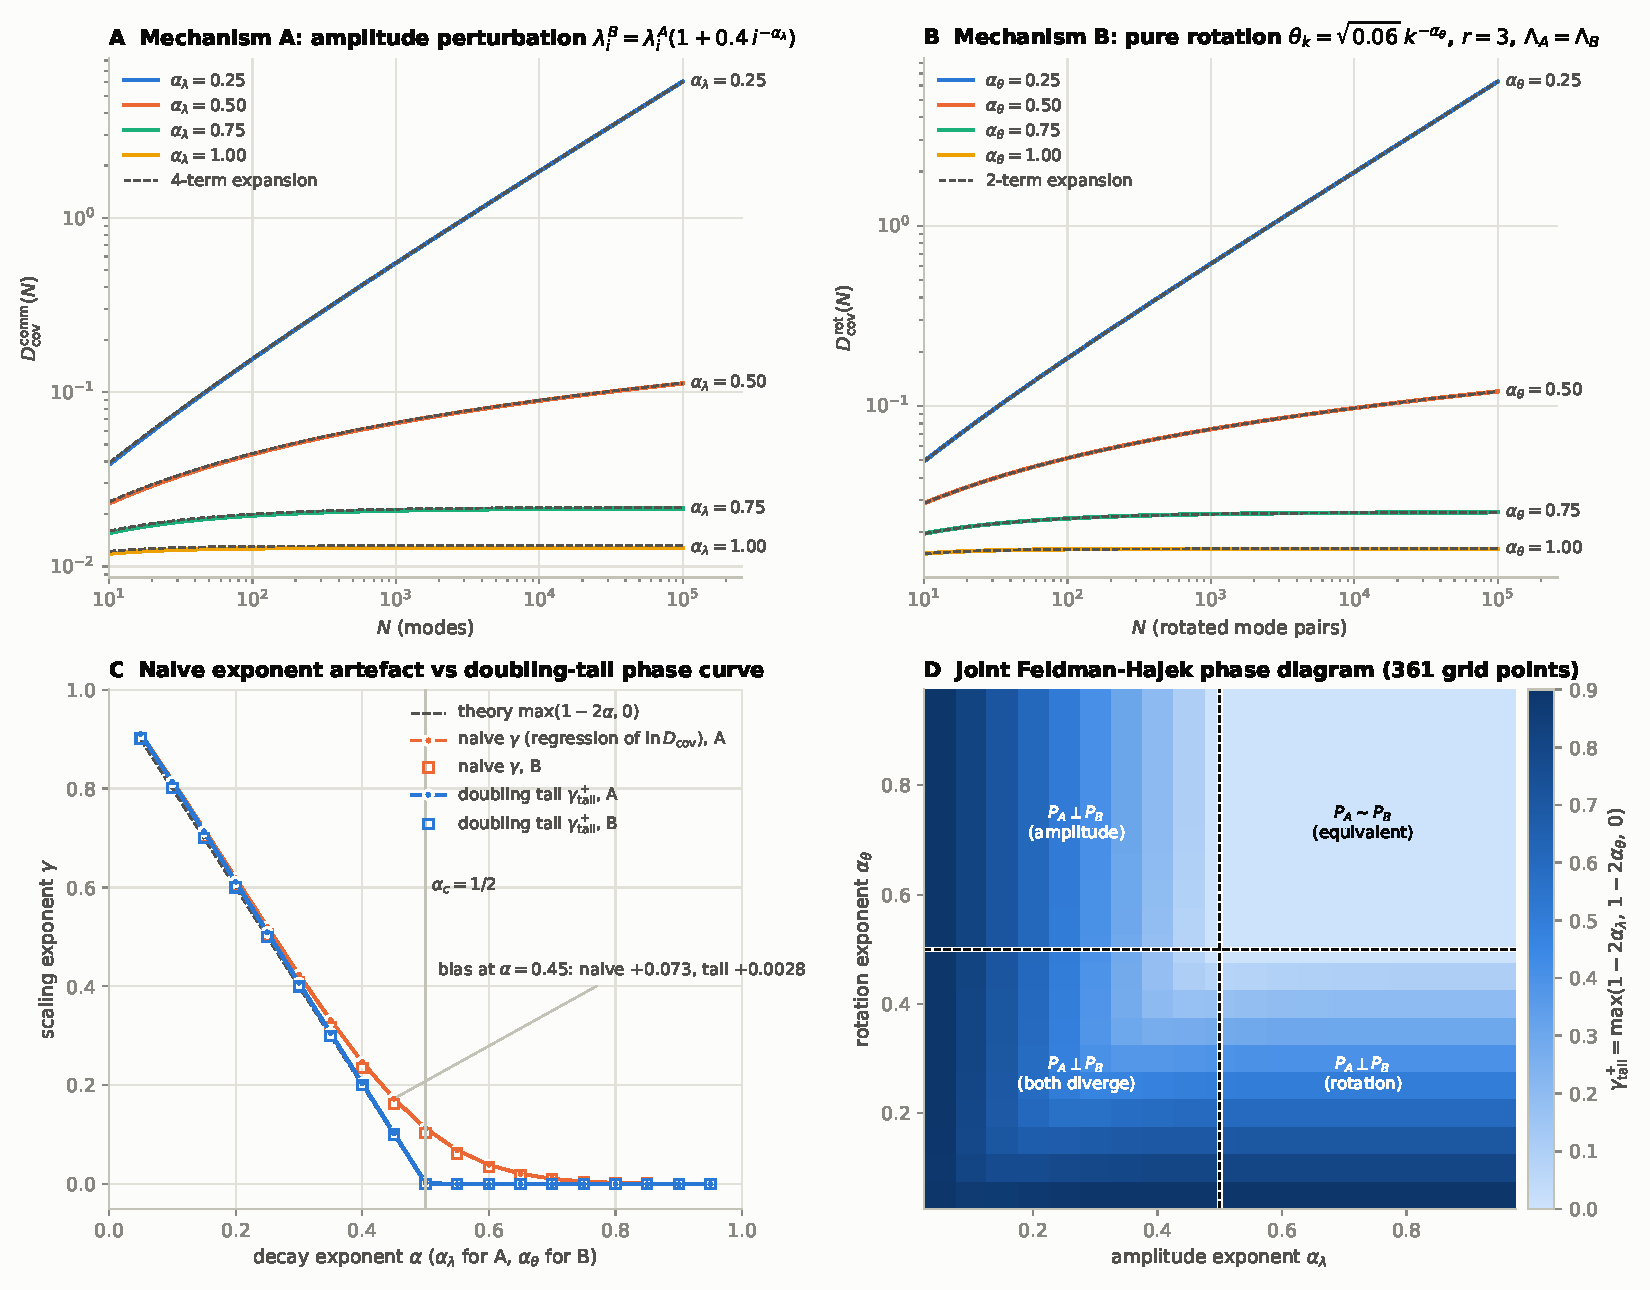
\includegraphics[width=\textwidth]{fig03_spectral_kakutani_criticality.pdf}
\caption{Spectral Kakutani criticality of covariance perturbations decaying along the mode index (file \texttt{fig03} in \texttt{figures/}).
\textbf{A.} Mechanism~A: $\Dcomm(N)$ on doubly logarithmic axes for $\alpha_\lambda\in\{0.25,0.5,0.75,1\}$ with the four-term expansion \eqref{eq:dAexp} summed (dashed) superposed: power-law divergence, logarithmic divergence, saturation at $D_\infty(0.75)=0.02157$ and $D_\infty(1)=0.01278$.
\textbf{B.} Mechanism~B: $\Drot(N)$ for the same exponents with the two-term expansion \eqref{eq:dBexp}: the same three regimes, with saturation at $0.02577$ and $0.01613$, although every eigenvalue is unchanged.
\textbf{C.} The naive exponent (orange) is a smooth curve through $\alpha_c$---$0.1729$ (A) and $0.1619$ (B) at $\alpha=0.45$, $0.113$ and $0.104$ at $\alpha=\tfrac12$---while the doubling-tail exponent $\gtail^+$ (blue) is the sharp kink $\max(1-2\alpha,0)$ of Theorem~\ref{thm:tail}; filled circles are Mechanism~A, open squares Mechanism~B, and at $\alpha=0.45$ the two estimators differ by $+0.073$ against $+0.0028$ (A).
\textbf{D.} The joint phase diagram of Theorem~\ref{thm:phase}: measured $\gtail^+$ on the $19\times19$ grid, with the boundaries $\alpha_\lambda=\tfrac12$ and $\alpha_\theta=\tfrac12$ (dashed). The lower-right quadrant is the rotation-driven singular phase of cryptic iso-spectral allostery; the upper-right quadrant is the only equivalent phase.}
\label{fig:phase}
\end{figure}

%%%%%%%%%%%%%%%%%%%%%%%%%%%%%%%%%%%%%%%%%%%%%%%%%%%%%%%%%%%%%%%%%%%%%%%%%%%%%%%
\clearpage
\section{Self-critical assessment}
\label{sec:assessment}

We separate what is established from what is not.

\subsection*{Established unconditionally}
The closed-form coefficients \eqref{eq:dA} and the exact block formulas \eqref{eq:dB} and \eqref{eq:blockexact} (Propositions~\ref{prop:A}, \ref{prop:B}, Lemma~\ref{lem:block}); the series representation \eqref{eq:Dseries}, the three-regime asymptotics with their constants, and the spectral Feldman--H\'ajek dichotomy at $\alpha_c=\tfrac12$ for each mechanism (Theorem~\ref{thm:threeregime}); the exact cancellation of the Euler--Maclaurin constants by the doubling increment and the limit \eqref{eq:gtaillimit} (Theorem~\ref{thm:tail}); the refined slope formula \eqref{eq:refined} (Theorem~\ref{thm:refined}); the parity statements and the shift formula \eqref{eq:dgamma} (Theorem~\ref{thm:parity}(1)--(3)); the joint phase criterion \eqref{eq:phase} (Theorem~\ref{thm:phase}).

\subsection*{Conditional or incomplete}
The cross-over formula of Corollary~\ref{cor:crossover} treats the slowly varying rotational coefficient $\kappa_k$ through the remainder; its full analytic form reproduces the grid to $4\times10^{-4}$, but the leading closed form is only accurate to $0.013$ where the Euclidean amplitude shift is large. The model spectra are idealised: $r$ is the same for every pair, the mode pairing is fixed in advance, and no mode matching problem arises. The identification of $\alpha_\lambda$ and $\alpha_\theta$ with measurable properties of a real protein is not attempted. As in Papers I--II, $N\to\infty$ is an idealisation and every finite-$N$ affinity is strictly positive; the theorems concern scaling with $N$.

\subsection*{Relation to the literature}
The Feldman--H\'ajek theorem \cite{Feldman1958,Hajek1958} and Kakutani's theorem \cite{Kakutani1948} are the two dichotomies used; the affine-invariant geometry of $\PN$ and its geodesic (log-Euclidean in the commuting case) coordinates are classical \cite{Bhatia2007,Pennec2006}; the Euler--Maclaurin expansion of $H_N(s)$ is standard \cite{Apostol1999,Titchmarsh1986}. Principal-component (essential-dynamics) analysis of protein covariances \cite{Amadei1993} supplies the modes on which the two mechanisms act, and the ensemble view of allostery with its cryptic sites \cite{Bowman2012,Motlagh2014,Nussinov2013} supplies the premise. We are not aware of a treatment of covariance-spectrum perturbations as a Feldman--H\'ajek critical phenomenon, nor of the doubling estimator in this context; a literature check remains advisable.

\begin{table}[ht]
\centering\small
\caption{Assessment of Paper III.}
\label{tab:assessment}
\begin{tabular}{@{}p{0.5\textwidth}p{0.18\textwidth}p{0.24\textwidth}@{}}
\toprule
Item & Status & Where \\
\midrule
Exact per-mode / per-pair contributions and their series & established & Props.~\ref{prop:A}, \ref{prop:B} \\
Three-regime asymptotics, constants, $\alpha_c=\tfrac12$ for A and B & established & Thm.~\ref{thm:threeregime} \\
Agreement with data: $3\times10^{-12}$ at $N\ge100$ & verified numerically & Tables~\ref{tab:benchA}, \ref{tab:benchB} \\
Doubling tail cancels $\zeta(2\alpha)$; $\gtail\to1-2\alpha$ on $(0,1)$ & established & Thm.~\ref{thm:tail} \\
Refined naive-slope formula reproduces $\gnaive$ to $10^{-4}$ & established / verified & Thm.~\ref{thm:refined}, Table~\ref{tab:scaling} \\
Geodesic parity; Euclidean pull-back; shift formula \eqref{eq:dgamma} & established & Thm.~\ref{thm:parity} \\
$\gtail(0.45)$: $+0.1028$ (A), $+0.1001$ (A-geo), $+0.1001$ (B) & verified numerically & Table~\ref{tab:threeway} \\
Joint phase criterion $\min(\alpha_\lambda,\alpha_\theta)\le\tfrac12$; $361/361$ points & established / verified & Thm.~\ref{thm:phase}, Table~\ref{tab:phase} \\
Two-power-law cross-over on the joint grid; all four characteristic entries; $4\times10^{-4}$ on $361$ points & established / verified & Cor.~\ref{cor:crossover} \\
Empirical covariances: noise, mode matching, Marchenko--Pastur & open & Problem (1) \\
\bottomrule
\end{tabular}
\end{table}

\subsection*{Open problems and next steps}
\begin{enumerate}[label=(\arabic*),leftmargin=*]
\item \emph{Empirical covariance matrices.} A covariance estimated from $T$ frames of a molecular-dynamics trajectory of $N$ coordinates has, for $T/N$ of order one, a bulk of noise eigenvalues distributed by the Marchenko--Pastur law \cite{MarchenkoPastur1967,Laloux1999}, and the corresponding eigenvectors are random. Both fingerprints are then contaminated exactly in the high-index tail that decides the dichotomy: the amplitude ratios $\eta_i$ of bulk modes are pure noise, and the rotation angles $\theta_k$ of bulk modes are close to $\pi/2$ irrespective of the ligand. The next step is to filter the bulk (keep the eigenvalues above the Marchenko--Pastur edge $\sigma^2(1+\sqrt{N/T})^2$, or apply shrinkage) before evaluating $\Dtail$, and to determine how the decay exponents $\alpha_\lambda,\alpha_\theta$ of the retained modes can be estimated with a controlled bias.
\item \emph{Mode matching.} For real spectra the pairing of modes between $\CA$ and $\CB$ is not given; the rotation fingerprint should be defined through an optimal assignment (or through the principal angles between the subspaces spanned by the first $k$ modes), and Theorem~\ref{thm:phase} should be restated for that definition.
\item \emph{The rotational coefficient.} Corollary~\ref{cor:crossover} absorbs the $k$-dependence of $\kappa_k=\kappa(r;x_{1,k},x_{2,k})$ into a remainder; an explicit expansion of $\bar\kappa$ in powers of $k^{-\alpha_\lambda}$ would turn the leading closed form \eqref{eq:convex} into a two-term formula of the same accuracy as the full analytic fit.
\item \emph{Beyond fixed anisotropy.} Allow $r_k$ to vary with $k$ and $\theta_k$ to couple non-adjacent modes; the block formula \eqref{eq:blockexact} generalises to any $2\times2$ invariant subspace, but the Givens structure does not.
\end{enumerate}

\subsection*{Reproducibility}
\begin{sloppypar}
All results are generated by two scripts in \texttt{code/}: \texttt{exp03\_spectral\_kakutani\_criticality.py} (data, figure, acceptance tests) and \texttt{paper03\_compute\_tables.py} (series coefficients, Euler--Maclaurin predictions, limits, the geodesic variant, the shift formula, and the table bodies; its text summary is \texttt{results/paper03\_tables\_summary.txt}); the first runs in about a minute, the second in seconds, with NumPy, Matplotlib and mpmath. The paper and its \LaTeX{} source (\texttt{paper/}), the raw data (\texttt{data/}), the figure (\texttt{figures/}) and the derived tables (\texttt{results/}) are archived under DOI \href{https://doi.org/10.5281/zenodo.23015709}{10.5281/zenodo.23015709} and maintained at \url{https://github.com/Ruqing1963/kakutani-statistical-pharmacology-III}.
\end{sloppypar}

\subsection*{Funding}
This project was supported by the National Natural Science Foundation of China (No.~22464010), the Guangxi Natural Science Foundation of China (No.~2025GXNSFAA069294), and the 2025 Bagui Youth Top Talent Project.

\begin{thebibliography}{99}
\bibitem{Amadei1993} A.~Amadei, A.~B.~M. Linssen and H.~J.~C. Berendsen, \emph{Essential dynamics of proteins}, Proteins \textbf{17} (1993), 412--425.
\bibitem{Apostol1999} T.~M. Apostol, \emph{An elementary view of Euler's summation formula}, Amer. Math. Monthly \textbf{106} (1999), 409--418.
\bibitem{Bhatia2007} R.~Bhatia, \emph{Positive Definite Matrices}, Princeton University Press, Princeton, 2007.
\bibitem{Bowman2012} G.~R. Bowman and P.~L. Geissler, \emph{Equilibrium fluctuations of a single folded protein reveal a multitude of potential cryptic allosteric sites}, Proc. Natl. Acad. Sci. USA \textbf{109} (2012), 11681--11686.
\bibitem{ChenChen2026I} Z.~Chen and R.~Chen, \emph{Statistical pharmacology via Kakutani dichotomy I: the marginal drug Kakutani index and the $\alpha_c=1/2$ criticality theorem in high-dimensional conformational ensembles}, 2026, DOI 10.5281/zenodo.23005921.
\bibitem{ChenChen2026II} Z.~Chen and R.~Chen, \emph{Statistical pharmacology via Kakutani dichotomy II: the correlated Kakutani index, the 99.95\% covariance dominance theorem, and spectral fingerprints of cryptic allostery}, 2026, DOI 10.5281/zenodo.23012217.
\bibitem{Feldman1958} J.~Feldman, \emph{Equivalence and perpendicularity of Gaussian processes}, Pacific J. Math. \textbf{8} (1958), 699--708.
\bibitem{Hajek1958} J.~H\'ajek, \emph{On a property of normal distributions of any stochastic process}, Czechoslovak Math. J. \textbf{8} (1958), 610--618.
\bibitem{Kakutani1948} S.~Kakutani, \emph{On equivalence of infinite product measures}, Ann. of Math. (2) \textbf{49} (1948), 214--224.
\bibitem{Laloux1999} L.~Laloux, P.~Cizeau, J.-P. Bouchaud and M.~Potters, \emph{Noise dressing of financial correlation matrices}, Phys. Rev. Lett. \textbf{83} (1999), 1467--1470.
\bibitem{MarchenkoPastur1967} V.~A. Marchenko and L.~A. Pastur, \emph{Distribution of eigenvalues for some sets of random matrices}, Math. USSR Sb. \textbf{1} (1967), 457--483.
\bibitem{Motlagh2014} H.~N. Motlagh, J.~O. Wrabl, J.~Li and V.~J. Hilser, \emph{The ensemble nature of allostery}, Nature \textbf{508} (2014), 331--339.
\bibitem{Nussinov2013} R.~Nussinov and C.-J. Tsai, \emph{Allostery in disease and in drug discovery}, Cell \textbf{153} (2013), 293--305.
\bibitem{Pennec2006} X.~Pennec, P.~Fillard and N.~Ayache, \emph{A Riemannian framework for tensor computing}, Int. J. Comput. Vis. \textbf{66} (2006), 41--66.
\bibitem{Titchmarsh1986} E.~C. Titchmarsh, \emph{The Theory of the Riemann Zeta-Function}, 2nd ed., revised by D.~R. Heath-Brown, Oxford University Press, 1986.
\end{thebibliography}

\end{document}
